\documentclass[10pt,landscape]{article}
\usepackage[utf8]{inputenc}
\usepackage{multicol}
\usepackage{calc}
\usepackage{ifthen}
\usepackage[portrait]{geometry}
\usepackage{amsmath,amsthm,amsfonts,amssymb}
\usepackage{mathtools}
\usepackage{color,graphicx,overpic}
\usepackage{hyperref}
\usepackage{enumerate}
\usepackage{etoolbox} % Required for \appto.
\usepackage{centernot}
\usepackage{xargs}
\usepackage{ifthen}
\usepackage[shortlabels]{enumitem}
\usepackage{xcolor}
\usepackage{multirow}
\usepackage{dcolumn}
\usepackage{pgfplots}
\pgfplotsset{compat=1.18}
\newcommand{\mbf}{\mathbf}
\newcommand{\bs}{\boldsymbol}
\newcommand{\lb}{\lambda}
\newcommand{\f}{\frac}
\newcolumntype{2}{D{.}{}{2.0}}

\DeclarePairedDelimiter\abs{\lvert}{\rvert}

%%%%%%%%%%%%%%%%%%%%%%%%%%%%%%%%%%%%%%%%%%%%%%%%%%%%%%%%%%%%%%%%%%%%%%%%%%%%%%%%%%%%%%%%%%%%%%

% Define emphasis to be bold face and italic.
\DeclareTextFontCommand{\emph}{\bfseries\em}

% Removes most of whitespace above and below equations.
\newcommand{\zerodisplayskips}{%
  \setlength{\abovedisplayskip}{-5pt}% Default: 12pt plus 3pt minus 9pt
  \setlength{\belowdisplayskip}{3pt}% Default: 0pt plus 3pt
  \setlength{\abovedisplayshortskip}{-5pt}% Default: 12pt plus 3pt minus 9pt
  \setlength{\belowdisplayshortskip}{3pt}% Default: 7pt plus 3pt minus 4pt
}
\appto{\normalsize}{\zerodisplayskips}
\appto{\small}{\zerodisplayskips}
\appto{\footnotesize}{\zerodisplayskips}

%%%%%%%%%%%%%%%%%%%%%%%%%%%%%%%%%%%%%%%%%%%%%%%%%%%%%%%%%%%%%%%%%%%%%%%%%%%%%%%%%%%%%%%%%%%%%%%
% Theorem Environment Setup %
%%%%%%%%%%%%%%%%%%%%%%%%%%%%%%%%%%%%%%%%%%%%%%%%%%%%%%%%%%%%%%%%%%%%%%%%%%%%%%%%%%%%%%%%%%%%%%%
\usepackage{amsthm}

% New environments for definitions and theorems. These will let us put in the
% exact reference to the definition/theorems in the notes, e.g.
%
% \begin{definition}{5.1.1}
%     ...
% \end{definition}
%
% to create a definition with title "Definition 5.1.1", referencing the
% definition with the same number in the notes.
\newenvironment{definition}[1] {
    \par\addvspace{\topsep}
    \noindent\textbf{Definition #1}.
    \ignorespaces
}

\newenvironmentx{theorem}[2][\empty] {

    \newcommand{\Title}{Theorem}

    \ifthenelse{ \equal{#2}{\empty} }{
        % Only one argument supplied, don't need parantheses.
        \par\addvspace{\topsep}
        \noindent\textbf{\Title\  #1}.
        \ignorespaces
    }{
        % Two arguments supplied, show in parantheses.
        \par\addvspace{\topsep}
        \noindent\textbf{\Title\  #1} (#2).
        \ignorespaces
    }
}

\newenvironmentx{lemma}[2][\empty] {

    \newcommand{\Title}{Lemma}

    \ifthenelse{ \equal{#2}{\empty} }{
        % Only one argument supplied, don't need parantheses.
        \par\addvspace{\topsep}
        \noindent\textbf{\Title\  #1}.
        \ignorespaces
    }{
        % Two arguments supplied, show in parantheses.
        \par\addvspace{\topsep}
        \noindent\textbf{\Title\  #1} (#2).
        \ignorespaces
    }
}

\newenvironmentx{proposition}[2][\empty] {

    \newcommand{\Title}{Proposition}

    \ifthenelse{ \equal{#2}{\empty} }{
        % Only one argument supplied, don't need parantheses.
        \par\addvspace{\topsep}
        \noindent\textbf{\Title\  #1}.
        \ignorespaces
    }{
        % Two arguments supplied, show in parantheses.
        \par\addvspace{\topsep}
        \noindent\textbf{\Title\  #1} (#2).
        \ignorespaces
    }
}

\newenvironmentx{corollary}[2][\empty] {

    \newcommand{\Title}{Corollary}

    \ifthenelse{ \equal{#2}{\empty} }{
        % Only one argument supplied, don't need parantheses.
        \par\addvspace{\topsep}
        \noindent\textbf{\Title\  #1}.
        \ignorespaces
    }{
        % Two arguments supplied, show in parantheses.
        \par\addvspace{\topsep}
        \noindent\textbf{\Title\  #1} (#2).
        \ignorespaces
    }
}

\newenvironmentx{remark}[2][\empty] {

    \newcommand{\Title}{Remark}

    \ifthenelse{ \equal{#2}{\empty} }{
        % Only one argument supplied, don't need parantheses.
        \par\addvspace{\topsep}
        \noindent\textbf{\Title\  #1}.
        \ignorespaces
    }{
        % Two arguments supplied, show in parantheses.
        \par\addvspace{\topsep}
        \noindent\textbf{\Title\  #1} (#2).
        \ignorespaces
    }
}

\newenvironmentx{example}[2][\empty] {

    \newcommand{\Title}{Example}

    \ifthenelse{ \equal{#2}{\empty} }{
        % Only one argument supplied, don't need parantheses.
        \par\addvspace{\topsep}
        \noindent\textbf{\Title\  #1}.
        \ignorespaces
    }{
        % Two arguments supplied, show in parantheses.
        \par\addvspace{\topsep}
        \noindent\textbf{\Title\  #1} (#2).
        \ignorespaces
    }
}

\newenvironmentx{exercise}[2][\empty] {

    \newcommand{\Title}{Exercise}

    \ifthenelse{ \equal{#2}{\empty} }{
        % Only one argument supplied, don't need parantheses.
        \par\addvspace{\topsep}
        \noindent\textbf{\Title\  #1}.
        \ignorespaces
    }{
        % Two arguments supplied, show in parantheses.
        \par\addvspace{\topsep}
        \noindent\textbf{\Title\  #1} (#2).
        \ignorespaces
    }
}

\newenvironmentx{question}[2][\empty] {

    \newcommand{\Title}{Question}

    \ifthenelse{ \equal{#2}{\empty} }{
        % Only one argument supplied, don't need parantheses.
        \par\addvspace{\topsep}
        \noindent\textbf{\Title\  #1}.
        \ignorespaces
    }{
        % Two arguments supplied, show in parantheses.
        \par\addvspace{\topsep}
        \noindent\textbf{\Title\  #1} (#2).
        \ignorespaces
    }
}

%%%%%%%%%%%%%%%%%%%%%%%%%%%%%%%%%%%%%%%%%%%%%%%%%%%%%%%%%%%%%%%%%%%%%%%%%%%%%%%%%%%%%%%%%%%%%%%
% Commands for Mathematical Typesetting %
%%%%%%%%%%%%%%%%%%%%%%%%%%%%%%%%%%%%%%%%%%%%%%%%%%%%%%%%%%%%%%%%%%%%%%%%%%%%%%%%%%%%%%%%%%%%%%%

% Redefine \leq and \geq to something nicer looking:
\renewcommand{\leq}{\leqslant}
\renewcommand{\geq}{\geqslant}

% Inner Product:
\DeclareRobustCommand{\InnerProduct}[2]{
    \ifmmode
        \left( #1,#2 \right)
    \else
        \GenericError{\space\space\space\space}
        {Attempting to use \InnerProduct outside of math mode}
    \fi
}

% Vector Norm: 
\DeclareRobustCommand{\Norm}[1]{
    \ifmmode
        \left\lVert #1 \right\rVert
    \else
        \GenericError{\space\space\space\space}
        {Attempting to use \Norm outside of math mode}
    \fi
}

% Image of Function:
\DeclareMathOperator{\im}{im}

% Interior of a Curve:
\DeclareMathOperator{\Int}{Int}

% Exterior of a Curve:
\DeclareMathOperator{\Ext}{Ext}

% Proof Hint:
\newcommand{\Hint}{\textit{Hint: }}

% Real numbers:
\newcommand{\R}{\mathbb{R}}

% Rational numbers:
\newcommand{\Q}{\mathbb{Q}}

% Natural numbers:
\newcommand{\N}{\mathbb{N}}

% Integers:
\newcommand{\Z}{\mathbb{Z}}

% Distance:
\newcommand{\di}[2]{d\left(#1, #2\right)}

% Solution command:
\newcommand{\soln}{\textbf{Solution: }}

% Put a number or letter in parenthesis, bold
\newcommand{\bpar}[1]{\textbf{(#1)}}

% Domain shorthand:
\newcommand{\dom}{\text{dom}}

%%%%%%%%%%%%%%%%%%%%%%%%%%%%%%%%%%%%%%%%%%%%%%%%%%%%%%%%%%%%%%%%%%%%%%%%%%%%%%%%%%%%%%%%%%%%%%%
% PAGE SETUP %
%%%%%%%%%%%%%%%%%%%%%%%%%%%%%%%%%%%%%%%%%%%%%%%%%%%%%%%%%%%%%%%%%%%%%%%%%%%%%%%%%%%%%%%%%%%%%%%

% This sets page margins to .5 inch if using letter paper, and to 1cm
% if using A4 paper. (This probably isn't strictly necessary.)
% If using another size paper, use default 1cm margins.
\ifthenelse{\lengthtest { \paperwidth = 11in}}
    { \geometry{top=.5in,left=.5in,right=.5in,bottom=.5in} }
    {\ifthenelse{ \lengthtest{ \paperwidth = 297mm}}
        {\geometdry{top=1cm,left=1cm,right=1cm,bottom=1cm} }
        {\geometry{top=1cm,left=1cm,right=1cm,bottom=1cm} }
    }

% Turn off header and footer
\pagestyle{empty}

% Redefine section commands to use less space
\makeatletter
\renewcommand{\section}{\@startsection{section}{1}{0mm}%
                                {-1ex plus -.5ex minus -.2ex}%
                                {0.5ex plus .2ex}%x
                                {\normalfont\large\bfseries}}
\renewcommand{\subsection}{\@startsection{subsection}{2}{0mm}%
                                {-1explus -.5ex minus -.2ex}%
                                {0.5ex plus .2ex}%
                                {\normalfont\normalsize\bfseries}}
\renewcommand{\subsubsection}{\@startsection{subsubsection}{3}{0mm}%
                                {-1ex plus -.5ex minus -.2ex}%
                                {1ex plus .2ex}%
                                {\normalfont\small\bfseries}}
\makeatother

% Define BibTeX command
\def\BibTeX{{\rm B\kern-.05em{\sc i\kern-.025em b}\kern-.08em
    T\kern-.1667em\lower.7ex\hbox{E}\kern-.125emX}}

% Don't print section numbers
\setcounter{secnumdepth}{0}


\setlength{\parindent}{0pt}
\setlength{\parskip}{0pt plus 0.5ex}

\setlist[itemize]{leftmargin=0.5cm}
\setlist[enumerate]{leftmargin=0.5cm}

%My Environments
%\newtheorem{example}[section]{Example}
% -----------------------------------------------------------------------

%%%%%%%%%%%%%%%%
% FIGURES %
%%%%%%%%%%%%%%%%
\usepackage{lipsum}
\newenvironment{Figure}
  {\par\medskip\noindent\minipage{\linewidth}}
  {\endminipage\par\medskip}

%%%%%%%%%%%%%%%%%%%%%%%%%%%%%%%%%%%%%%%%%%%%%%%%%%%%%%%%%%%%%%%%%%%%%%%%%%%%%%%%%%%%%%%%%%%%%%%
% SECTION AND SUBSECTION TITLES %
%%%%%%%%%%%%%%%%%%%%%%%%%%%%%%%%%%%%%%%%%%%%%%%%%%%%%%%%%%%%%%%%%%%%%%%%%%%%%%%%%%%%%%%%%%%%%%%
\usepackage[explicit]{titlesec}
\usepackage[normalem]{ulem}
\usepackage{lipsum}

\titleformat{\section}
  {\normalfont\Large}{}{0em}{\uline{\thesection#1}}
\titleformat{name=\section,numberless}
  {\normalfont\Large}{}{0em}{\uline{#1}}

\titleformat{\subsection}
  {\normalfont\normalsize\bfseries}{}{0em}{\uline{\thesection#1}}
\titleformat{name=\subsection,numberless}
  {\normalfont\normalsize\bfseries}{}{0em}{\uline{#1}}

%%%%%%%%%%%%%%%%%%%%%%%%%%%%%%%%%%%%%%%%%%%%%%%%%%%%%%%%%%%%%%%%%%%%%%%%%%%%%%%%%%%%%%%%%%%%%%%
% BEGINNING OF THE DOCUMENT %
%%%%%%%%%%%%%%%%%%%%%%%%%%%%%%%%%%%%%%%%%%%%%%%%%%%%%%%%%%%%%%%%%%%%%%%%%%%%%%%%%%%%%%%%%%%%%%%

\begin{document}
\raggedright
\footnotesize
\begin{multicols}{2}

%%%%%%%%%%%%%%%%%%%%%%%%%%%%%%%%%%%%%%%%%%%%%%%%%%%%%%%%%%%%%%%%%%%%%%%%%%%%%%%%%%%%%%%%%%%%%%%
% MULTICOLS PARAMETERS %
%%%%%%%%%%%%%%%%%%%%%%%%%%%%%%%%%%%%%%%%%%%%%%%%%%%%%%%%%%%%%%%%%%%%%%%%%%%%%%%%%%%%%%%%%%%%%%%
% multicols parameters
% These lengths are set only within the two main columns
%\setlength{\columnseprule}{0.25pt}
\setlength{\premulticols}{1pt}
\setlength{\postmulticols}{1pt}
\setlength{\multicolsep}{1pt}
\setlength{\columnsep}{2pt}
\setlength{\columnseprule}{0.4pt} % For vertical lines separating columns.

%%%%%%%%%%%%%%%%%%%%%%%%%%%%%%%%%%%%%%%%%%%%%%%%%%%%%%%%%%%%%%%%%%%%%%%%%%%%%%%%%%%%%%%%%%%%%%%
% TYPING STARTS HERE %
%%%%%%%%%%%%%%%%%%%%%%%%%%%%%%%%%%%%%%%%%%%%%%%%%%%%%%%%%%%%%%%%%%%%%%%%%%%%%%%%%%%%%%%%%%%%%%%
\begin{center}
    \Large{Honours Differential Equations Cheatsheet}\\
    \footnotesize{Callum Burgher}\\ 
\end{center}
\normalsize

\section{1. Prior Knowledge}
\begin{itemize}
   
    \item Linear equations (Integrating factor method):\\The ODE in standard form: $\frac{dy}{dx}+P(x)y=Q(x)$
    \begin{enumerate}
        \item Let $I.F=e^{\int P(x)\ dx}$ 
        \item Then, $y(I.F)=\int I.F \ Q(x)\ dx$ and solve for $y$
    \end{enumerate}

\item Separable equations: An ODE that can be written: $\frac{dy}{dx}=g(x)h(y)$\\Solution is found by $\int \frac{1}{h(y)}\ dy = \int g(x)\ dx$

\item Homogeneous equations: The ODE: $\frac{dy}{dx}=f(x,y)$ is called homogeneous if $f(x,y)$ can be expressed as a function of the ratio $\frac{y}{x}$ only. (i.e., $f(x,y)$). \\ To solve: Change the dependent variable to $v(x)=\frac{y}{x}$, then use separation of variables

\item Exact equations: The ODE: $M(x,y) + N(x,y)\frac{dy}{dx}=0$ is called exact if there exists a function $\psi(x,y)$ s.t\\ 
$\frac{\partial \psi}{\partial x}= M(x,y)$ and $\frac{\partial \psi}{\partial y}= N(x,y)$. (iff $\frac{\partial M}{\partial y} = \frac{\partial N}{\partial x}$) \\ If the ODE is exact then it can be written as $\frac{d}{dx}\psi(x,y)$ and integrating gives $\psi(x,y)=c$

\item Integrating factors: Take a non-exact ODE, sometimes can be made exact if we multiply by an integrating factor $\mu(x,y).$ \\ New ODE is exact iff $\frac{\partial}{\partial y}(\mu M)=\frac{\partial}{\partial x}(\mu N)$
\end{itemize}

Linear Homogeneous ODEs with constant coefficients: \\Form, $ay''+by'+cy=0$ 
\begin{enumerate}
    \item First set up the characteristic eqn: $ar^2+br+c=0$. Now there are 3 cases 
    \begin{enumerate}
        \item[(i)] If there are two real valued and distinct roots, $r_1$ and $r_2$, then $y(t)=C_1e^{r_1t}+C_2e^{r_2t}$

        \item[(ii)] If there is only one double root, $r$, then $y(t)=C_1e^{rt}+C_2te^{rt}$

        \item[(iii)] If there are complex-valued conjugate roots, $r=a\pm  ib$: $y(t)=e^{at}(C_1\cos{bt}+C_2\sin{bt})$
    \end{enumerate}

   \item Plug in initial conditions and solve (if appropriate)
    
\end{enumerate}

Linear Non-Homogeneous ODEs with constant coefficients:\\
In the form $ay''+by'+cy=g(t)$.

\begin{enumerate}
    \item Answer is in form: $y_c(t)+y_p(t)=0$
    \item Find $y_c(t)$ as homogeneous with RHS=0
    \item Find $y_p(t)$ by 'guessing'
    \begin{enumerate}
        \item[Case(i)] If $g(t)=Me^{kt}$
        \item[Case(ii)] If $g(t)= M\cos{kt} + N\sin{kt}$
        \item[Case(iii)] If $g(t)= a_nt^n+a_{n-1}t^{n-1}+\cdots+a_1t+a0$ 
        \item[Case(iv)] If $g(t)$ is a product of the above functions then take the corresponding product of functions
        \item[Case(v)] If $g(t)$ is a sum of any of the above then find each solution separate and add both into the general solution at end
    \end{enumerate}
\end{enumerate}

\section{2. Systems of ODEs}

\textbf{Thm 1.8:}If the function \( F \) is continuous in a region\\ 
\[
[\alpha_1, \beta_1] \times \dots \times [\alpha_n, \beta_n] \times [\alpha, \beta]
\]
containing \((\bf{x}_0, 0)\), and if all partial derivatives \(\frac{\partial F_i}{\partial x_j}\), \(i, j = 1, \dots, n\), are also continuous there, then there exists a \(\delta > 0\) such that the given initial value problem has a unique solution for \(t \in [-\delta, \delta]\).

\textbf{Thm 1.9:} (Principle of Superposition)\\ If $\{\textbf{x}^{j}(t)\}, j =1,\dots,p$ is a set of solutions, \\$$\textbf{x}(t)\sum_{j=1}^pc_j\textbf{x}^{(j)}(t), \quad c_j\in \mathbb{R}$$ is also a solution\\
\bigskip
\textbf{Wronskian:}
\begin{equation*}
   	 W[y_1,...,y_n] = \begin{vmatrix}
   	   y_1       &  y_2  & \dots &  y_n \\ 
  	    y'_1       &  y'_2 & \dots &  y'_n\\
    	  \dots  & \dots&      & \dots    \\
   	   y^{(n-1)}_1   & y^{(n-1)}_2 & \dots & y^{(n-1)}_n\\ 
   	 \end{vmatrix} 
 	 \end{equation*}
	  The functions $\{y_i\}$ form a fundamental set of solutions if $ W \neq 0$ (i.e. if they're linearly independent. Then any solution can be written as their linear combination. If $W(x_0) \neq 0$ then $W(x) \neq 0 \quad \forall x \in [\alpha, \beta].$ 

\textbf{Thm 1.11:} (Abel's Theorem). If $W(t_0)\neq 0$ for some $t_0,$ then $W(t)\neq 0$ for all $\alpha\le t\le \beta$ \\
\textbf{Thm 1.12:} (Abel's Formula) The wronskian satisfies \\$$W'(t)=tr(P(t))W(t)=(P_{11}+\cdots +P_{nn})W(t)$$ Hence, $$W(t)=e^{\int_{t_0}^t trP(s)ds} W(t_0).$$
\textbf{Trace:}$tr(A)$ sum of all of the diagonal elements of $A$
\begin{itemize}
    \item Transforming $n$th order ODE into a system of first-order ODEs: \begin{enumerate}
        \item Define n new indep variables $x_1=y, x_2=y', \dots, x_n = y^{(n-1)} $

        \item Derivatives: $x_1'=x_2, \dots, x_{n-1}' = x_n, \ x_n' = y^n$
        \item The system is $x_1'=x_2,\dots, x_n'=F(x_1,\dots,x_{(n-1)},t)$
    \end{enumerate}
    
    \item \textbf{Fundamental Matrices:} A fundamental matrix $\Psi(t)$ is an $n\times n$ matrix with fundamental solutions $\mbf{x}^{(i)}$: Properties 

    \begin{enumerate}
        \item det$\Psi(t)=W(t)\neq 0$
        \item $\mbf{x}(t) = \Psi(t)\mbf{c}$
        \item $\Psi'(t)=A\Psi(t)$ ($\Psi(t)$ is a solution of the system of ODEs)
        \item $\mbf{x}(t) = \Psi(t)\Psi^{-1}(t_0)\mbf{x}_0$ solves $\mbf{x}'(t)= A\mbf{x}(t),$ with $\mbf{x}(t_0)=\mbf{x}_0$
     \end{enumerate}
     \item \textbf{Matrix Exponentiation}\\
       \begin{align*}
 	 e^{At} &= \sum_{n=0}^\infty \frac{(At)^n}{n!} = \mathbb{I}+At+\frac{A^2t^2}{2!}+\frac{A^3t^3}{3!}... \\
  	 &= \lim_{n \rightarrow \infty} \left(\mathbb{I}+\frac{1}{n}A\right)^n
  \end{align*}
  \begin{itemize}
  	\item $\mathbf{x}(t) = e^{At}\mathbf{x}_0 \iff e^{At} = \Psi(t)\Psi^{-1}(t_0)$
	\item$e^{At} = \Psi(t)$ for $\Psi(0) = \mathbb{I}$
  \end{itemize}

    
Let $\frac{d\mathbf{x}}{dt} = A\mathbf{x}$ and consider the matrix $T$ with eigenvectors $\xi^{(i)}$ as columns. The matrix $AT$ has columns equal to $A\xi^{(1)} = r_i\xi^{(i)}$, so \\
  \begin{align*}
  AT &= \begin{pmatrix} 
       r_1 \xi_1^{(1)}    & \dots &  r_n\xi_1^{(n)}   \\
      \vdots   & \ddots   &  \vdots \\
      r_1 \xi_n^{(1)}    & \dots & r_n \xi_n^{(n)}  \\
  \end{pmatrix} 
  = T \begin{pmatrix} 
        r_1  & 0& \dots &  0 \\
      	0 &  r_2 & \dots    & 0 \\
     	\vdots & \vdots & \ddots & \vdots \\
     	0 & 0 & \dots &r_n \\
  	\end{pmatrix} \\ &= T \text{diag}(r_1,...,r_n) = TD \implies D = T^{-1}AT .
  \end{align*}
  
Then $\mathbf{x} = T\mathbf{y} \implies \frac{d\mathbf{y}}{dt} = D\mathbf{y}$ and in the new variables, the solution is\\
\vspace{0.05cm}

$$\mathbf{y}_i = e^{r_it} \begin{pmatrix} 0 \\  . \\ 1 \\ 0 \\ . \\0 \end{pmatrix} \quad \text{1 $i$-th component.}$$

Thus its fundamental matrix equals $Q(t) = e^{Dt} = \text{diag}(e^{r_1t},...,e^{r_nt})$. 
The fundamental matrix in the original variables $\mathbf{x}$ is $\Psi(t) = TQ(t)$ and the exponential matrix is $e^{At} = \Psi(t)\Psi^{-1}(0) = TQT^{-1}$. Only works if $A$ is diagonalisable. If we have eigenvalues with geometric multiplicity $<$ algebraic multiplicity, we cannot diagonalise!

 \subsection{Homogeneous Solution Method}
    Given a system in the form $\frac{d\textbf{x}}{dt}=A\textbf{x}$, find \textbf{x}$_h$ by finding $r_1, r_2$ as your eigenvalues, and then find corresponding $\xi_1, \xi_2.$ Then, one of the following occurs
    \begin{enumerate}
        \item $r_1\neq r_2$ are real $\implies \textbf{x}_h = c_1e^{r_1t}\xi_1 + c_2e^{r_2t}\xi_2.$
        \item $r_1^*=r_2=u+iv\implies\textbf{x}_h=e^{ut}(\textbf{a}\cos(vt)+\textbf{b}i\sin(vt)).$ Then split into real and imaginary parts \textbf{x}$_{h1}= \textbf{h}_1+i\textbf{h}_2$ to get the homogeneous solution $\textbf{x}_h = c_1\textbf{h}_1+c_2\textbf{h}_2$
        \item $r_1=r_2$ then you must find the generalised eigenvector \begin{itemize}
        
        \item One solution is $\mathbf{x}_1 = e^{\lambda t} \xi$.
		\item Second solution is of the form $\mathbf{x}_2 = te^{\lambda t} \xi + e^{\lambda t} \eta$ with $ (A-\lambda \mathbb{I}) \eta = \xi$.
		\item (Third solution is of the form $\mathbf{x}_3 = \frac{t^2}{2}e^{\lambda t} \xi + te^{\lambda t} \eta + e^{\lambda t} \zeta$ with $ (A-\lambda \mathbb{I}) \boldsymbol{\zeta} = \eta \cdots$.)
        \end{itemize}
	\end{enumerate}

	\textbf{Connection to matrix methods} Build a matrix $T$ out of $\xi, \eta, (\zeta)$, then $T^{-1}AT = J$ where $J$ is an upper triangular matrix (Jordan form). We can then proceed as if it was $D$ above. The exponential has the form \\
	$$ e^{J_{\lambda}t} = \begin{pmatrix} e^{\lambda t} & te^{\lambda t} \\ 0 & e^{\lambda t} \end{pmatrix}. $$$\textbf{x}_h=c_1te^{rt}\xi+c_2e^{rt}\xi+c_3e^{rt}\eta.$

\subsection{Nonhomogeneous Systems of ODEs}
\bigskip$$ \mathbf{x}' = A\mathbf{x}+\mathbf{g}(t)$$
The general solution is of the form\\ $$ \mathbf{x}(t) = \sum_i c_i\mathbf{x}^{(1)}(t) + \mathbf{x}_{\text{par}}(t). $$

The difference of any two solutions of the non-homogeneous equation $\textbf{x}(t)=P(t)\textbf{x}(t)+\textbf{g}(t)$ satisfies the associated homogeneous equation $\textbf{x}(t)=P(t)\textbf{x}(t)$

    \subsubsection{Diagonalisation}
	Introduce change of variables $\mathbf{x}=T\mathbf{y}$, so we have\\
	$$ T\mathbf{y}' = AT\mathbf{y} + \mathbf{g}(t) \implies \frac{d\mathbf{y}}{dt} = D\mathbf{y} + T^{-1}\mathbf{g} = D\mathbf{y}+\mathbf{h}.$$
    Where $D$ is the matrix with eigenvalues on diagonal.\\
	This leads to a system of $n$ decoupled equation which we solve by direct integration:\\
	$$ y'_i = r_iy_i + h_i \implies y_i(t) = c_i e^{r_i t} + e^{r_i t}\int_{t_0}^t e^{-r_is}h_i(s)ds.$$
	General solution in the original variables equals $\mathbf{x}(t) = T\mathbf{y}(t)$.
	In case the matrix is not diagonalisable, find its Jordan form and proceed in a similar way (with $J$ instead of $D$). Note that we will need to integrate from the bottom up. 

		\subsubsection{Method of Undetermined Coefficients}
		Works if $\mathbf{g}(t)$ is built out of polynomials and exponentials (real or complex). Same rules apply with the exception that if $\mathbf{g}(t) = \mathbf{u}e^{\lambda t}$ where $\lambda$ is an eigenvalue of $A$ with multiplicity 1, then \\$$ \mathbf{x}_{\text{par}} = te^{\lambda t}\mathbf{a}+e^{\lambda t} \mathbf{b}. $$
		If the multiplicity is $n$, we must write $\mathbf{x}_{\text{par}} = e^{\lambda t}\sum_{i=0}^n t^i \mathbf{a}_i.$

		\subsubsection{Variation of Parameters}
		If $A = P(t)$ is not constant, we look for solutions to the non-homogeneous part of the form \\$$ \mbf{x}(t) = \Psi(t)\mbf{u}(t).$$ Introducing this to the system gives\\ $$ \f{d\mbf{x}}{dt} = \Psi'(t)\mbf{u}(t) +\Psi(t)\f{d\mbf{u}}{dt} = P(t)\Psi(t)\mbf{u}(t)+\mbf{g}(t).$$
 		Remembering $\Psi' = P(t)\Psi$, \\$$ \Psi \f{d\mbf{u}}{dt} = \mbf{g}(t) \implies \f{d\mbf{u}}{dt} = \Psi^{-1}\mbf{g} \implies \mbf{u}(t) $$$$ =\int_{t_0}^t \Psi^{-1}(s)\mbf{g}(s)ds +\mbf{f}$$
 		Thus the general solution is \\$$ \mbf{x}(t) = \Psi(t)\Psi^{-1}(t_0)\mathbf{x}_0 + \Psi(t)\int_{t_0}^t \Psi^{-1}(s)\mbf{g}(s)ds.$$
\end{itemize}
\section{3. Non-Linear Systems of ODEs}
\subsection{Qualitative Theory of ODEs}
 Consider a nonlinear autonomous system (i.e. $F,G$ have no explicit time dependence) \\$$ \f{dx}{dt} = F(x,y), \quad  \f{dy}{dt} = G(x,y).$$

 	\subsection{Critical Points} 
	A point $\mbf{x}_0 =(x_0,y_0)$ is a critical point if $F(x_0,y_0) = G(x_0,y_0) = 0$.
 	Locally, around any critical point, nonlinear ODEs $\approx$ linear ODEs. Use Taylor expansions (for $F$ and $G$):\\
 	\begin{align*} 
		F(x,y) = F(x_0,y_0) + \partial_x F(x_0,y_0)(x-x_0)\\ + \partial_y F(x_0,y_0)(y-y_0) +  \eta_1(x,y)
	\end{align*}
	where $\displaystyle\f{\eta_1(x,y)}{||\mbf{x}-\mbf{x_0}||} \rightarrow 0$ as $(x,y) \rightarrow (x_0,y_0)$. Linear approximation consists of dropping $\eta_1$. \\
	Introduce new variables $u_1 \equiv x-x_0$,  $u_2 \equiv y-y_0$. These satisfy \\
	$$ \f{d\mbf{u}(t)}{dt} = 
	\begin{pmatrix}
		 \partial_x F(x_0,y_0) & \partial_y F(x_0,y_0) \\
		 \partial_x G(x_0,y_0) & \partial_y G(x_0,y_0)
	 \end{pmatrix} \begin{pmatrix} u_1 \\ u_2 \end{pmatrix} =  A\mbf{u}.$$
$A$ is the Jacobian matrix.

Drawing eigenvectors on phase diagrams \begin{enumerate}
    \item \textbf{Positive} eigenvalue $=$ \textbf{travelling away} from critical point
    \item \textbf{Negative} eigenvalue $=$ \textbf{travelling towards} critical point
    \item \textbf{Trajectories} tend spin towards the eigenvector with largest eigenvalue
\end{enumerate}
\textbf{TABLE ON BACK}

A node is proper if it has independent eigenvectors and improper if there is only one unique eigenvector.
To determine whether the motion is clockwise or anticlockwise (centre), we must look to the original linear system:\\
\[
\mathbf{x}'(t) = \begin{pmatrix} a & b \\ c & d \end{pmatrix} \mathbf{x}(t).
\]
If \( b - c > 0 \), the motion is clockwise; if \( b - c < 0 \), the motion is anticlockwise.

	 A critical point $\mbf{x}_0$ is \textbf{stable} if $\forall \epsilon$, $\exists \delta>0$ s.t. every solution $\mbf{x} = \phi(t)$ with $||\phi(0)-\mbf{x}_0|| < \delta$ at $t=0$ satisfies $||\phi(t)-\mbf{x}_0|| < \epsilon$, $\forall t >0$.\\

     \textbf{Unstable} If $\exists \varepsilon>0 , \forall \delta>0 , \exists \bf{x}(t)$ that satisfies $||\bf{x}(0)-\bf{x}_0|| < \delta$ but for which $\exists t>0$ so that $||\bf{x}(t)-\bf{x}_0||\ge \varepsilon$\\
     \vspace{0.1cm}
	 A critical point $\mbf{x}_0$ is asymptotically stable if it is stable and the solution $\mbf{x} = \phi(t)$ is forced to approach $\mbf{x}_0$ as $t \rightarrow \infty$.
 
	Sometimes a nonlinear ODE system has an exact phase portrait given by \\
 	\vspace{-0.1cm}
  	$$ \left. \begin{array}{ll}
		\f{dx}{dt} = F(x,y) \\ \f{dy}{dt} = G(x,y)
                \end{array}
              \right\} \implies \f{dy}{dx} = \f{G(x,y)}{F(x,y)} \implies H(x,y) = c. $$

\subsection{Stability of Non-linear Systems}
Given a system described by\\
$$
\begin{cases}
x' = F(x, y) \\
y' = G(x, y)
\end{cases}
$$
we can transform it into a system of ODEs of the form\\
$$
\begin{pmatrix}
u' \\
v'
\end{pmatrix}
=
\begin{pmatrix}
\frac{\partial F}{\partial x}(x^*) & \frac{\partial F}{\partial y}(x^*) \\
\frac{\partial G}{\partial x}(x^*) & \frac{\partial G}{\partial y}(x^*)
\end{pmatrix}
\begin{pmatrix}
u \\
v
\end{pmatrix}
+
\begin{pmatrix}
\eta_1 \\
\eta_2
\end{pmatrix}
$$
which becomes a linear system if we ignore the perturbation\\
$$
\begin{pmatrix}
\eta_1 \\
\eta_2
\end{pmatrix}.
$$
It is tempting to make conclusions on the stability of the non-linear system based on the behavior of the linearized system. This is valid, except for the center for which we cannot determine the stability of based solely from the linearised system.

\subsubsection{Implicit Trajectories}
For the system \begin{align*}
    x'&=F(x,y)\\
    y'&=G(x,y).
\end{align*}
First find $\frac{dy}{dx} = \frac{G(x,y)}{F(x,y)}$ giving a first order ODE, if this can be integrated, sep of var. then we can use this method to solve the ODE. This makes implicit trajectories easier to plot . (Rare)
\subsection{Non-Linear Methods}
\subsubsection{Lyapunov's Theory}
\begin{itemize}

	 \item Let $E(x,y)$ be defined on a domain $D$ containing (0,0). \\
     \begin{itemize}
 	\item $ E(x,y)$ is \emph{positive (negative) definite} if  $ E(0,0) = 0$ and  $ E(x,y) >0$ $\forall(x,y)\in D$ ($ E(x,y) < 0$ $\forall(x,y)\in D$). \\
  	\item $ E(x,y)$ is \emph{positive (negative) semi-definite} if  $ E(0,0) = 0$ and  $ E(x,y) \ge 0$ $\forall(x,y)\in D$. ($ E(x,y) \le 0$ $\forall(x,y)\in D$). 
    \end{itemize}
	
  \item \textbf{Theorem 3.11} (Lyapunov Stability Theorem) Given an autonomous system with critical point (0,0), if $\exists E(x,y)$ continuous with continuous first partial derivatives, positive definite and for which $\f{dE}{dt}$ is negative definite on some domain $D$ containing (0,0) then (0,0) is asymptotically stable. If $\f{dE}{dt}$ is negative semi-definite $\implies$ (0,0) is stable (at the non-linear level). $E(x,y)$ is called \emph{Lyapunov function}. \\
  
   \item \textbf{Theorem 3.12} (Lyapunov Instability Theorem) Given an autonomous system with critical point (0,0), assume $\exists E(x,y)$ continuous with continuous first partial derivatives, such that $E(0,0) = 0$ and that in every neighbourhood of (0,0) $\exists$ at least one point $(x_1,y_1)$ where $E(x_1,y_1)$ is positive (negative). If $\exists$ some domain $D$ containing (0,0) where $\f{dE}{dt}$ is positive definite (negative definite) on $D \implies$ (0,0) is an unstable critical point.

        
\end{itemize}
    
    	\subsubsection{Limit Cycles}
	\begin{itemize}
	    
    \item Periodic solutions: $f(x+T) = f(x)$ $\forall x$ (the smallest possible $T$ is fundamental period). Trajectories form closed curves. 
    \item A linear combination or product of functions with the same period $T$ also have period $T$. 
    \item Limit cycles are periodic solutions such that at least one other non-closed trajectory asymptotically approaches them as \( t \to \infty \) (or \( t \to -\infty \), or both).
    \item Let $F(x,y), G(x,y)$ have continuous first partial derivatives in some domain $D$. The we have the following:\\ \begin{itemize}
	
\item \textbf{Theorem 3.18}  A closed trajectory must necessarily enclose at least one critical point. If it encloses only one critical point, it cannot be a saddle point. (i.e. no critical points in $D \implies$ no closed trajectories in $D$; if $\exists$ a unique critical point in $D$ and it is a saddle $\implies$ no closed trajectories in $D$).\\
	
        \item \textbf{Theorem 3.19} Let $D$ be simply connected (i.e. without holes). If $\partial_xF + \partial_yG$ has the same sign in $D \implies$ there are no closed trajectories in $D$.\\
        
        \item \textbf{Poincar\'e-Bendixon Theorem} Let $R$ consist of a bounded subdomain of $D$ and its boundary. Suppose $R$ has no critical points. If a certain trajectory lies entirely in R, then this trajectory either is a periodic (closed) trajectory or spirals towards one. Either way,  $\exists$ a closed trajectory.
        \end{itemize}
           \end{itemize}

    \section{4. Fourier Series}
    	\textbf{Inner Product} \\ 
	\begin{align*}
		(u(x),v(x)) &\equiv \int_{-L}^L u(x)v(x)dx \\
		(u(x),v(x)) &\equiv \int_{\alpha}^{\beta} u^*(x)v(x)dx \quad \text{ (complex functions)} 
        \end{align*}
        The set $ \{1,  \sin{\f{n \pi x}{L}}, \cos{\f{m \pi x}{L}} \} $ forms an orthogonal basis. If $S_n(x) = \sin{\f{n \pi x}{L}}, S_m(x) = \sin{\f{m \pi x}{L}}, C_n(x) = \cos{\f{n \pi x}{L}}, C_m(x) = \cos{\f{m \pi x}{L}}, C_0 = 1$, then \\
        \small
        \vspace{0.2cm}
        \begin{align*}
        		\left. \begin{array}{ll}
			(S_m,S_n) &= 0  \\
          		(S_n,S_n)&= L 
                \end{array}
              \right\} \implies (S_m,S_n) = L \delta_{mn} \quad m,n \neq 0 \\
          	\left. \begin{array}{ll}
			(C_m,C_n) &= 0 \\
           		(C_n,C_n) &= L 
                \end{array}
              \right\} \implies (C_m,C_n) = L \delta_{mn} \quad m,n \neq 0 \\
	(S_m,C_n) = (S_n, C_n) = (C_0,C_m) = (C_0,S_m) = 0, \quad (C_0,C_0) = 2L. \end{align*}

    Where $\delta_{mn}$ is the Kronecker Delta function: \\
\normalsize
    $$\delta_{mn} = \begin{cases}
        1,\quad n= m,\\
        0, \quad n\neq m.
    \end{cases}$$

	A periodic function with period $2L$ can be expressed as \emph{Fourier series} \\
	\begin{align*} 
		f(x) &= \f{a_0}{2} + \sum_{n=1}^{\infty} \left( a_n \cos{\f{n \pi x}{L}} + b_n \sin{\f{n \pi x}{L}} \right) \\
		 &= \sum_{n = - \infty}^{\infty} c_n e^{i n \pi x / L} 
	\end{align*}

    \textbf{Fourier Convergence Theorem:} For piecewise continuous functions the series converges to $f(x)$ $\forall x$ where $f(x)$ is continuous. At discontinuities, the series converges to $ \f{f(x^+)+f(x^-)}{2}$, not to $f(x)$ - Gibbs phenomenon.

		\subsubsection{Euler-Fourier Formulas} Projecting the function onto orthogonal basis gives \\
		\begin{align*} 
			\f{a_0}{2} &= \f{1}{2L} \int_{-L}^L f(x) dx \equiv \langle f(x) \rangle = c_0\\
   		        a_n  &= \f{1}{L} \int_{-L}^L f(x) \cos{\f{n \pi x}{L}} dx, \quad n=0,1,2,... \\
   		        b_n &= \f{1}{L} \int_{-L}^L f(x) \sin{\f{n \pi x}{L}} dx \\
    		        c_n &= \f{a_n - ib_n}{2}, \quad c_{-n} =  \f{a_n + ib_n}{2} \quad (n>0) \\
   		        c_n &=  \f{1}{2L} \int_{-L}^L f(x)e^{-\f{i n \pi x}{L}}dx, \quad n \in \mathbb{Z}
		\end{align*}

     Complex trig: $\cos(x) = \frac{e^{ix}+ e^{-ix}}{2}$ and $\sin(x) = \frac{e^{ix}-e^{-ix}}{2i}$
        
		Even functions ($f(-x)=f(x)$) only have cosine coefficient series. Odd functions ($f(-x) = -f(x)$) only have sine coefficient series. Due to symmetries, even/odd functions only require information about half the interval $[0,L]$. (See integration section on even and odd functions)

		\subsubsection{Parseval's Theorem}
		\begin{align*}
			(f,f) &= \int_{-L}^L |f(x)|^2 dx = 2L \sum_{n = - \infty}^{\infty} |c_n|^2 \\
			 &= L \left[ \f{|a_0|^2}{2} + \sum_{n=1}^{\infty} (|a_n|^2 + |b_n|^2) \right] 
 		\end{align*}

\section{5. PDEs by separation of Variables}

$\textbf{General Form:} \quad X'' + \lambda X = 0$

\begin{itemize}
    \item \textbf{Case 1:} \(\lambda > 0\)\\
    \[
    X(x) = A\cos(kx) + B\sin(kx), \quad k = \sqrt{\lambda}.
    \]
    Oscillatory solutions (e.g., sine and cosine).

    \item \textbf{Case 2:} \(\lambda = 0\)
    \[
    X(x) = Ax + B.
    \]
    Linear solutions.

    \item \textbf{Case 3:} \(\lambda < 0\)\\
    \[
    X(x) = A\cosh(kx) + B\sinh(kx), \quad k = \sqrt{|\lambda|}.
    \]
    Exponential solutions written in terms of hyperbolic functions.

    If $X'' -\lambda X = 0$ instead, change g.s for case 1 and case 3
\end{itemize}

\textbf{SUMMARY}
\begin{itemize}
 	\item Assume separation of variables $u(x,t) = X(x)T(t)$.
	\item Introduce one (or more) separation parameter $\lb$.
	\item Solve eigenvalue problem(s): quantisation of $\lb$ (depends on boundary / initial conditions).
	\item Write the most general solution as a linear combination of all solutions to the eigenvalue boundary problems.
	\item Identify any undetermined coefficients using initial conditions.
 \end{itemize}
 
		\subsubsection{Heat Equation}
		$$ \partial_t u =\alpha^2 \partial_x^2 u, \quad \alpha > 0 $$
		\begin{itemize}
			\item initial condition: $u(x,0) = f(x)$, $0\le x \le L $\\
			\item boundary conditions: $u(0,t), u(L,t)$, $t >0$ 
		\end{itemize}
        $\textbf{Notation:} \quad \partial_t u \equiv \frac{\partial u}{\partial t} \equiv u_t, \quad \partial_x^2 u \equiv \frac{\partial^2 u}{\partial x^2} \equiv u_{xx}$

		
		\textbf{Homogeneous boundary conditions} $u(0,t) =  u(L,t) = \underline{0}$\\
		\begin{align*}
			u(x,t) = X(x)T(t) \implies X''+\lb X &= 0 \\ T'+\alpha^2 \lb T &= 0 
		\end{align*}
		\begin{align*}
			X_n(x) &= \sin{\f{n \pi x}{L}}, \quad n=1,2,3,... \quad \lb_n = \f{n^2 \pi^2 }{L^2} \\
			T_n &= e^{-\f{n^2 \pi^2 \alpha^2 t}{L^2}}
		\end{align*}\\
		$$ u(x,t) = \sum_{n=1}^{\infty} c_nX_n(x)T_n(t) = \sum_{n=1}^{\infty} c_n e^{-\f{n^2 \pi^2 \alpha^2 t}{L^2}} \sin{\f{n \pi x}{L}} $$
		$$ c_n = \f{2}{L} \int_0^L f(x)  \sin{\f{n \pi x}{L}} dx $$

		\textbf{Nonhomogeneous boundary conditions} $u(0,t) =  T_1, u(L,t) = T_2$. \\
		Map problem to one with homogeneous boundary conditions. Define time independent function $g(x) = \lim_{t \rightarrow \infty}u(x,t).$ \\
		$$g(x) = T_1 +(T_2-T_1)\f{x}{L} \implies u(x,0) = f(x)-g(x)$$

        Then $\partial_t g = 0$ and it is easy to solve for $g(x)$. The original problem has the form $u(x,y) = g(x) + w(x,t)$ ($w(x)$ satisfies a homogeneous set of boundary conditions with different initial value function). \\
		$$ c_n = \f{2}{L} \int_0^L (f(x)-g(x))  \sin{\f{n \pi x}{L}} dx$$
		$$ u(x,t)  = T_1 + (T_2-T_1)\f{x}{L}  + \sum_{n=1}^{\infty} c_n e^{-\f{n^2 \pi^2 \alpha^2 t}{L^2}} \sin{\f{n \pi x}{L}} $$

		\textbf{Insulated ends} $X'(0) = X'(L) = 0$ \\ Process is the same but this time the result is a cosine series. 

		\subsubsection{Wave Equation}
		$$\partial_t^2 u = a^2 \partial_x^2 u \quad \text{ $a$ = wave speed}$$ \\ $(a^2 = \frac{T}{\rho}$  where  $T$ is the tension (force) and  $\rho$  is the mass per unit length) $\implies a$ \ has the units of length/time- that is, of velocity)
		\begin{itemize}
			\item initial position: $u(x,0) = f(x)$ \\
			\item initial velocity $u_t(x,0) = g(x)$ \\
			\item fixed ends: $u(0,t) = u(L,t) = 0 $ 
		\end{itemize}
		
		\textbf{String with initial position} No initial velocity, so $u_t(x,0) = 0 \implies T'(0) = 0$. $X_n$ and $c_n$ are same as homogeneous heat equation.
		$$ u(x,t) = \sum_{n=1}^{\infty} c_nX_n(x)T_n(t) = \sum_{n=1}^{\infty} c_n \sin{\f{n \pi x}{L}} \cos{\f{n \pi a t}{L}} $$

		\textbf{String with initial velocity} No initial position, so $u(x,0) = 0 \implies T(0) = 0$. We find that\\ $$ T_n(t) = \sin{\f{n \pi a t}{L}}$$
		$$ u(x,t) = \sum_{n=1}^{\infty} c_n \sin{\f{n \pi x}{L}} \sin{\f{n \pi a t}{L}} $$\\
		$$ c_n = \f{2}{n \pi a} \int_0^L g(x)  \sin{\f{n \pi x}{L}} dx $$

		\textbf{String with initial position and velocity} Let $v(x, t)$ be the solution for the vibrating string with no initial velocity ($g(x) = 0$). Let $w(x, t)$ be the solution for the string with no initial displacement ($f(x) = 0$). Then $u(x, t) = v(x, t) + w(x, t).$

		\subsubsection{Laplace's Equation}
		$$ \nabla^2u \equiv \partial_x^2 u + \partial_y^2 u = 0 $$
		Dirichlet boundary conditions: $u(x,y)$ specified at the boundary. \\
        \textbf{Rectangle} Assume separation of variables $u(x,y) = X(x)Y(y)$. Then \\
		\begin{align*}
			X'' - \lb X = 0 \\
			Y'' + \lb Y = 0 
		\end{align*}
		Example : $u(x,0)=u(x,b)=0, u(0,y) =0, u(a,y) = f(y), 0 \le x \le a, 0 \le y \le b$\\
		$$ u(x,y) =  \sum_{n=1}^{\infty} c_n \sinh{\f{n \pi x}{b}} \sin{\f{n \pi y}{b}} $$
		$$ c_n  \sinh{\f{n \pi a}{b}}  = \f{2}{b} \int_0^b f(y)  \sin{\f{n \pi y}{b}} dy $$

		\textbf{Disc} Change coordinates:\\
		$$ \f{\partial^2 u }{\partial r^2} + \f{1}{r^2}\f{\partial^2u}{\partial \theta^2} + \f{1}{r}\f{\partial u }{\partial r} = 0$$
		Assume $u(r,\theta) = R(r)\Theta(\theta)$, then \\
		\begin{align*}
			r^2R'' +rR' = \lb R \\
			\Theta'' =  -\lb \Theta
		\end{align*}
		Example: $u(a,\theta) = f(\theta), x^2 + y^2 = a^2, 0 \le \theta \le 2\pi$ and $u(x,y) = \sqrt{x^2 + y^2} \le a$ \\
		Periodicity and boundedness determine:
		\begin{itemize}
			\item $\lb = 0$ allows a constant solution $u_0(r,\theta) = \f{c_0}{2}$.
			\item $\lb = n^2$ allows solutions of the form $u_n(r,\theta) = r^n (a_n \cos{n\theta} + b_n \sin{n\theta})$
		\end{itemize}
		$$ u(r,\theta) = \f{c_0}{2} + \sum_{n=1}^{\infty} r^n(e_n\cos{n\theta} + f_n \sin{n\theta} )$$
		$$ u(a,\theta) = f(\theta) =  \f{c_0}{2} + \sum_{n=1}^{\infty} a^n(e_n\cos{n\theta} + f_n \sin{n\theta} )$$\\
		$$ a^n e_n = \f{1}{\pi} \int_{-\pi}^{\pi} f(\theta)\cos{n\theta} d\theta $$\\
		$$ a^n f_n = \f{1}{\pi} \int_{-\pi}^{\pi} f(\theta)\sin{n\theta} d\theta $$

\section{6. Sturm-Liouville Theory}
    \subsection{Sturm-Liouville Boundary Problems}
		\textbf{Generalisation of the heat equation:} \\$$r(x)\partial_tu(x,t) = \partial_x[p(x)\partial_xu(x,t)]-q(x)u(x,t), \quad 0< x< 1$$

        with \begin{itemize}
            \item $\{p(x), p'(x), q(x), r(x)\}:$ real values, \textbf{continuous} on $x\in[0,1]$
            \item $p(x), r(x)> 0 \quad\forall x\in[0,1]$

            Separation of variables: $u(x,t) = X(x)T(t)$ yields

            $$r(x)X(x)\dot{T}(t) = [p(x)X'(x)]'T(t)-q(x)X(x)T(t)$$

            dividing by $r(x)X(x)T(t):$

            $$\frac{\dot{T}(t)}{T(t)}=\frac{[p(x)X'(x)]'}{r(x)X(x)}=-\lambda$$

            Thus, we are left with 2 ODEs: \\\begin{align*}
                \dot{T}(t)+\lambda T(t) &= 0\\
                [p(x)X'(x)]'-q(x)X(x)+\lambda r(x)X(x) &=0
            \end{align*}

            For 2nd ODE, define $X(x)\equiv y(x)$

            $$\text{i.e.,}\quad -[p(x)y'(x)]'+q(x)y(x) = \lambda r(x)y(x)$$

            and rewrite in terms of operator $L$:

            $$\text{i.e.,} \ L[y] = \lambda r(x)y(x)$$
        \end{itemize}

\textbf{Transforming ODEs into SL form:}
Begin with condition $[\mu(x)P(x)]' = \mu(x)Q(x)$, substitute what you know from $P(x)y'' + Q(x)y' + R(x)y = 0$, obtain $\mu'(x)$ and then integrate to find $\mu(x)$. Often in the form $\int\frac{\mu'(x)}{\mu(x)}dx =\dots \implies \ln(\mu(x)) = ...$. Then exponentiate\\
        \medskip
        \textbf{Defn 6.1 - Regular SL:} The eigenvalue ODE equation

        $$Ly = -[p(x)y']'+q(x)y = \lambda r(x)y, \quad 0\le x \le 1$$

        Subject to the boundary conditions:

        \begin{align*}
            a_1y(0)+a_2y'(0)&=0\\
            b_1y(1)+b_2y'(1)  &=0
        \end{align*}

        \textbf{Singular SL:} These are problems for which conditions on $p, q, r$ are satisfied $0<x<1$ but are not satisfied at $x=0$ and/or $x=1$
        
        \subsubsection{Homogeneous Problems}
		Consider differential equations of the form\\ $$[ p(x)y']' - q(x)y + \lb r(x)y = 0 $$
		Define the differential operator $L$ and rewrite the equation \\
		\begin{align*}
			L[y] &= -[ p(x)y']'  + q(x)y \\
			L[y] &= \lb r(x)y 
		\end{align*}
		$$a_1 y(0)+a_2y'(0) = 0 \quad b_1y(1) + b_2 y'(1) = 0$$
		All eigenvalues $\lb$ for which there are nontrivial solutions are real. If we have two eigenvalues $\lb_1$ and $\lb_2$ with $\lb_1 \neq \lb_2$ and corresponding eigenfunctions $\phi_1, \phi_2$ then 	$$ \langle \phi_1, \phi_2 \rangle = \int_0^1 r(x)\phi_1(x)\phi_2(x) dx = 0. $$
		That is, the pair is orthogonal with respect to the inner product defined by the Sturm-Liouville problem (w.r.t the weight function $r(x)$), denoted by the angled brackets to differentiate from the original inner product.  For each eigenvalue, there is a unique linearly independent eigenfunction. They form and infinite ordered sequence $\lb_1 < \lb_2 .. < \lb_n$ and $\lb_n \rightarrow \infty$. \\
		Eigenfunctions satisfying \\
        \footnotesize
        $$ \langle \phi_n, \phi_n \rangle = (\phi_m, r\phi_n) = \int_0^1 \phi_m(x)\phi_n (x) r(x) dx = \delta_{mn} =\begin{cases}
		    0 \quad \text{if} \ m\neq n\\
            1 \quad \text{if} \ m = n
		\end{cases} $$\normalsize are said to be normalised and form an orthonormal set w.r.t. $r(x)$. 
		A function $f(x)$ can be written as a sum of these eigenfunctions as follows:\\
		$$ f(x) = \sum_{n=1}^{\infty} c_n \phi_n(x) $$
		Multiplying by $r(x)\phi_m(x)$ and integrating gives the projection of $f(x)$ onto $\phi_m$. The overall aim of this section is to find $c_m$\\
		$$ \sum_{n=1}^{\infty} c_n  \int_0^1 r(x)\phi_m(x)\phi_n(x) dx = c_m $$
		$$ c_m = \int_0^1 r(x)\phi_m(x)f(x) dx= \langle f(x), \phi_m \rangle $$

        \textbf{Lagrange's Identity}\\ $$ \int_0^1 (L[u]v - uL[v]) dx = [-p(x)(u'(x)v(x) - u(x)v'(x))]_0^1 = 0$$
$$  (L[u],v) -(u,L[v]) = 0 $$

\subsection{Lagrange's Identity for singular SL problems}
\begin{itemize}
    \item Suppose S-L problem is singular at $x=0$ but not at $x=1$
    \item Consider \\$$\int_\varepsilon^1 \{L[u]v - uL[v]\}dx = -p(x)[u'(x)v(x)-u(x)v'(x)]_\varepsilon^1$$
    \item If $u, v$ satisfy the homogeneous boundary condition \\$$b_1y(1)+b_2y'(1)=0$$

    then\\
    $$u'(1)v(1) - u(1)v'(1) = -\frac{b_1}{b_2}u(1)v(1) + \frac{b_1}{b_2}u(1)v(1) = 0$$

    for $b_2\neq 0$, and likewise $u'(1)v(1)-u(1)v'(1) = 0$ for $b_2 = 0$. Thus, in the limit $\varepsilon\to 0$\\

    $$\int_0^1\{L[u]v-uL[v]\}dx = \lim_{\varepsilon\to 0}p(\varepsilon)[u'(\varepsilon)v(\varepsilon)-u(\varepsilon)v'(\varepsilon)]$$

    If $$\lim_{\varepsilon\to 0}p(\varepsilon)[u'(\varepsilon)v(\varepsilon)-u(\varepsilon)v'(\varepsilon)] = 0$$

   then Lagrange's identity yields\\ $$\int_0^1\{L[u]v-uL[v]\}dx = 0$$

    (the singular boundary problem is \textbf{self-adjoint}, and you can solve it as if it were a regular one

    
\end{itemize}
\subsection{Convergence Theorem}
We wish to consider the convergence of this series

$$\sum_{n=1}^\infty c_n\phi_n(x) \quad \text{with} \ c_n=\langle f, \phi_n\rangle$$

\textbf{Theorem 6.5} Assume $f$ and $f'$ are piecewise continuous. Then $\sum_{n=1}^\infty c_n\phi_n(x)$ converges: 
\begin{itemize}
    \item to $f(x)$ where $f$ is continuous,
    \item to $\frac{f(x_+)+f(x_-)}{2}$ (i.e., the midpoint of the left and right endpoints) elsewhere.
\end{itemize}

\subsubsection{Nonhomogeneous Problems}
\textbf{ODEs}
		$$ L[y] = -[ p(x)y']'  + q(x)y = \mu r(x)y + f(x) $$
		First look at the homogeneous problem $L[y] = \lb r(x)y$ with eigenvalues $\lb_1,\lb_2..$ and eigenfunctions $\phi_1,\phi_2...$ Assume the solution $y= \phi(x)$ can be written as 
		\begin{align*}
			\phi(x) &= \sum_{n=1}^{\infty} b_n\phi_n(x) \\
			c_n &= \int_0^1 f(x)\phi_n(x)dx \\
			b_n &= \f{c_n}{\lb_n - \mu} \\
			y &= \phi(x) = \sum_{n=1}^{\infty} \f{c_n}{\lb_n - \mu}\phi_n(x)
		\end{align*}
		If $c_n$ is zero then $b_n$ is arbitrary - infinitely many solutions. If $\lb_n = \mu$ for some $n$ and $c_n \neq 0 $ then there are no solutions. \\
\medskip
\textbf{PDEs:}

Consider the boundary problem:\\
$$
r(x) \frac{\partial u(x, t)}{\partial t} = \frac{\partial}{\partial x} \big[p(x) \frac{\partial u(x, t)}{\partial x}\big] - q(x) u(x, t) + F(x, t),
$$
where the solution satisfies the following boundary and initial conditions:\\
\begin{align*}
    \frac{\partial u(0, t)}{\partial x} - h_1 u(0, t) &= 0, \\
    \frac{\partial u(1, t)}{\partial x} + h_2 u(1, t) &= 0, \\
    u(x, 0) &= f(x).
\end{align*}


\begin{itemize}
    \item Assume the Sturm–Liouville boundary problem for \(X(x)\) is solved.
    \item There exists a set of eigenvalues \(\{\lambda_n\}\) associated with orthonormal eigenfunctions \(\{\Phi_n(x)\}\).
    \item Look for a solution to the non-homogeneous PDE by expanding \(u(x, t)\) in the basis of eigenfunctions:\\
    \[
    u(x, t) = \sum_{n=1}^\infty b_n(t)\Phi_n(x),
    \]
    where the set of unknowns is now the set \(\{b_n(t)\}\).
    \item Similarly, expand \(\frac{F(x, t)}{r(x)}\) in the same basis:\\
    \[
    \frac{F(x, t)}{r(x)} = \sum_{n=1}^\infty \gamma_n(t)\Phi_n(x),
    \]
    with the coefficients \(\gamma_n(t)\) given by:\\
    \[
    \gamma_n(t) = \int_0^1 r(x) \frac{F(x, t)}{r(x)} \Phi_n(x) \, dx.
    \]
\end{itemize}


Substituting the expansions into the non-homogeneous PDE:\\

\[
r(x) \sum_{n=1}^\infty \dot{b}_n(t) \Phi_n(x) = 
\sum_{n=1}^\infty b_n(t) \big[ -\big(p(x) \Phi_n'(x)\big)' + q(x) \Phi_n(x) \big] 
\]\\
\[+ r(x) \sum_{n=1}^\infty \gamma_n(t) \Phi_n(x).
\]

\
Since \(\Phi_n(x)\) satisfy the Sturm–Liouville boundary problem:\\
\[
-\big(p(x) \Phi_n'(x)\big)' + q(x) \Phi_n(x) = \lambda_n r(x) \Phi_n(x),
\]
we can simplify the PDE to:\\
\[
\sum_{n=1}^\infty \dot{b}_n(t) \Phi_n(x) = 
-\sum_{n=1}^\infty b_n(t) \lambda_n \Phi_n(x) + 
\sum_{n=1}^\infty \gamma_n(t) \Phi_n(x).
\]

From the substitution, we have:\\
\[
\sum_{n=1}^\infty \big[\dot{b}_n(t) + \lambda_n b_n(t) - \gamma_n(t)\big] \Phi_n(x) = 0.
\]
Using the orthonormality of the set \(\{\Phi_n(x)\}\), we can conclude that:\\
\[
\dot{b}_n(t) + \lambda_n b_n(t) = \gamma_n(t), \quad n = 1, 2, 3, \dots
\]
This is an infinite, countable set of linear first-order ordinary differential equations.

The ODEs can be solved using integrating factors. Multiply through by\\ \(\exp(\lambda_n t)\):
\[
\frac{d}{dt} \big(e^{\lambda_n t} b_n(t)\big) = e^{\lambda_n t} \gamma_n(t).
\]

Integrating both sides:\\
\[
\int_0^t \frac{d}{ds} \big(e^{\lambda_n s} b_n(s)\big) \, ds = \int_0^t e^{\lambda_n s} \gamma_n(s) \, ds.
\]

Solving, we get:\\
\[
b_n(t) = e^{-\lambda_n t} \int_0^t e^{\lambda_n s} \gamma_n(s) \, ds + e^{-\lambda_n t} \alpha_n,
\]
where \(\alpha_n = b_n(0)\).


\textbf{Mean Square Error:} Consider a function $f(x)$ and its expansion in an orthonormal basis \\

$$f(x) = \sum_{n=1}^\infty c_n\Phi_n(x)\quad \text{with} \quad c_m = \int_0^1 r(x)f(x)\Phi_m(x) dx$$

and consider a truncation of this series to finite $N$\\ 

$$S_N(x)= \sum_{n=1}^N c_n\Phi_n(x)$$

The mean square error involved in approximating $f(x)$ by $S_N(x)$ is 

$$c_N = \int_0^1 r(x)\left[f(x)-S_N(x)\right]^2\ dx.$$
\subsection{Examples of Sturm Liouville}

\textbf{Homogeneous ODE:}

Determine the normalized eigenfunctions of the following the boundary value problem

$$y''+\lambda y = 0, y'(0)=0, y(1) + y'(1) = 0.$$

Expand the function $f(x) = x, \ 0\le x<1$ in terms of these normalized eigenfunctions\\
\medskip
\textbf{Soln:} Since this is a SL bvp, $\lambda\in\mathbb{R}$. Use previous methods to check that there are no non-trivial solutions for $\lambda\le 0$. Thus, consider $\lambda > 0$. Therefore the general solution to the ODE is of the form \\

$$y(x) = c_1\cos(\sqrt{\lambda}x) + c_2\sin(\sqrt{\lambda}x).$$

The question is whether there is \textit{any} choice of $\{c_1,c_2\}$ compatible with the boundary question. First, 

$$y'(0) = 0\implies c_2 = 0, \implies y(x) = c_1\cos(\sqrt{\lambda}x)$$

Using this into the second boundary condition,

$$y(1)+y'(1) = 0 \implies \cos(\sqrt{\lambda}) = \sqrt{\lambda}\sin(\sqrt{\lambda}),  \text{i.e.,}  \ \tan(\sqrt{\lambda}) = \frac{1}{\sqrt{\lambda}}$$

Plotting these functions shows there exists an infinite number of solutions $\lambda_n$ for $n=1,2,\dots$ for each eigenvalue $\lambda_n$, there exists an eigenfunction $y(x)\propto \cos(\sqrt{\lambda}x)$

To obtain a set of orthonormal eigenfunctions $\Phi_n$, we consider the further constraint

$$(\Phi_n(x), \Phi_n(x)) = 1 \quad \text{with} \quad \Phi_n(x) = k_n\cos(\sqrt{\lambda_n}x).$$

The existence and form of the inner product follows from general theory. Thus, this condition reduces to 

$$k_n^2\int_0^1\cos^2(\sqrt{\lambda_n}x) \ dx = 1 \implies k_n = \frac{\sqrt{2}}{(1+\sin^2(\sqrt{\lambda_n}))^{1/2}},$$

where we used the constraint satisfied by the eigenvalue $\lambda_n$. This gives the normalized eigenfunctions \\ 

$$\Phi_n(x) = \frac{\sqrt{2}}{(1+\sin^2(\sqrt{\lambda_n}))^{1/2}}\cos(\sqrt{\lambda_n}x)$$


Once we have determined the basis of functions, we can expand $f(x) = x = \sum_{n=1}^\infty a_n\Phi_n(x).$ Using the orthonormality of the inner product, we find \\$$a_n = k_n\int_0^1x\cos(\sqrt{\lambda_n}x) \ dx = \sqrt{2}\frac{2\cos(\sqrt{\lambda_n} - 1}{\lambda_n(1+\sin^2(\sqrt{\lambda_n}))^{1/2}}$$


\bigskip 



\section{7. Laplace Transform}

The Laplace transform of $f(x)$ defined for $x\in [0, \infty)$ is \\$$ F(s) = \mathcal{L}\{f\}(s) \equiv \int_0^\infty e^{-sx} f(x) dx = \lim_{t \rightarrow \infty} \int_0^T e^{-sx}f(x)dx$$ Requires $f \in E$ ($f$ be of exponential type) - need $f(t)$ to be piecewise continuous on any $[0,T]$ where it is defined and $|f(x)| \le Ae^{Bx} \forall x \in [0,\infty)$ for some constants $A,B$. \\
It is a linear operation, i.e. \\$$\mathcal{L} \{c_1f_1(x) + c_2f_2(x)\}(s) = c_1 \mathcal{L} \{f_1(x)\} + c_2 \mathcal{L} \{f_2(x)\} .$$

If $f(x)$ is continuous on $[0,\infty)$ and $f,f' \in  E$ then \\ $$ \mathcal{L} \{f'(x)\} = s\mathcal{L}\{f(x)\} - f(0)$$\\
$$ \mathcal{L} \{f^{(n)}(x)\} = s^n\mathcal{L}\{f(x)\} - s^{n-1}f(0)-...-sf^{(n-2)}(0) - f^{(n-1)}(0)$$

Let $\mathcal{L}\{f(x)\}(s) = F(s)$:
\begin{enumerate}
 	\item \textbf{s-shift}:  $\mathcal{L}\{e^{-cx}f(x)\}(s) = F(s+c)$
	\item \textbf{x-shift}:  $\mathcal{L}\{f(x-c)\}(s) = e^{-sc} F(s)$ if $c\ge 0$ and $f(x)=0$ for $x<0$.
	\item \textbf{s-derivative}:  $\mathcal{L}\{xf(x)\}(s) = -F'(s)$ or in general $\mathcal{L}\{x^nf(x)\}(s) = (-1)^nF^{(n)}(s)$.
	\item \textbf{scaling}:  $\mathcal{L}\{f(cx)\}(s) = \frac{1}{c}F(\frac{s}{c})$,  $F(sc) = \frac{1}{c} \mathcal{L}\{f\left(\frac{x}{c}\right)\}$ if $c > 0$.

    \subsection{Unit Step Function}
		Given a function $f(t)$ defined for $t \ge0$, 
		\\$$ f(t)u_c(t) = \left\{
       		        \begin{array}{ll}
               		f(t) \quad \text{for}  \quad t\ge c\\
                  	0 \quad \text{for} \quad t < c
                		\end{array} \right. $$
                
              	$$ f(t)(u_a(t) -u_b(t)) = \left\{
                		\begin{array}{ll}
                  	f(t) \quad \text{for}  \quad t\in [a,b)\\
                  	0 \quad \text{for} \quad t \not\in [a,b)
                		\end{array} \right. $$
                
		\subsubsection{Dirac Distribution}
		$$ \delta(t) = 0 \quad \text{for} \quad t \neq 0, \quad \int_{-\infty}^{\infty} \delta(t)dt = 1 $$
		$$  \int_{-\infty}^{\infty} \delta(t - t_0)f(t)dt = f(t_0)$$

	\subsection{Convolution}
	Convolution is commutative, associative and distributive, but $(f*1) \neq f$ and $(f*f) \neq f^2$.\\
	$$ (f * g)(t) = \int_0^t f(\tau)g(t-\tau)d\tau $$\\
	$$ \mathcal{L} \{f*g\} = (\mathcal{L} \{f\})(\mathcal{L} \{g\}) $$
\textbf{SEE TABLE ON OTHER SIDE}

\end{enumerate}



\section{Trig Identities}

\begin{itemize}
    
    \item $\sin^2{(x)}+\cos^2{(x)}=1$
    \item $1+\tan^2(x)=\sec^2(x)$
    \item $1+\cot^2(x)=\csc^2(x)$
    \item $\sin{(x\pm y)}= \sin (x)\cos (y)\pm \cos (x)\sin (y)$
    \item $\cos{(x\pm y)}= \cos (x) \cos (y)\pm \sin (x)\sin (y)$
    \item $\sin(2x)= 2\sin(x)\cos(x)$
    \item $\cos(2x)= \cos^2(x)-\sin^2(x)$
    \item $\displaystyle\sin^2(x)= \frac{1-\cos(2x)}{2}$
    \item $\displaystyle\cos^2(x)= \frac{1+\cos(2x)}{2}$
    \item $\sin(-x)=-\sin(x)$
    \item $\cos(-x)=\cos(x)$
    \item $\tan(-x)=-\tan(x)$
    \item $\displaystyle\sec(x)= \frac{1}{\cos(x)}$
    \item $\displaystyle\csc(x)=\frac{1}{\sin(x)}$
    \item $\displaystyle\cot(x)=\frac{1}{\tan(x)}$ 
    \item $\displaystyle\sinh(x) = \frac{e^x - e^{-x}}{2}$
    \item $\displaystyle\operatorname{csch}(x) = \frac{1}{\sinh(x)} = \frac{2}{e^x - e^{-x}}$
    \item $\displaystyle\cosh(x) = \frac{e^x + e^{-x}}{2}$
    \item $\displaystyle\operatorname{sech}(x) = \frac{1}{\cosh(x)} = \frac{2}{e^x + e^{-x}}$
    \item $\displaystyle\tanh(x) = \frac{\sinh(x)}{\cosh(x)} = \frac{e^x - e^{-x}}{e^x + e^{-x}}$
    \item$\displaystyle\coth(x) = \frac{1}{\tanh(x)} = \frac{e^x + e^{-x}}{e^x - e^{-x}}$
    \item $\cosh^2(x) - \sinh^2(x) = 1$
    \item $\tanh^2(x) + \operatorname{sech}^2(x) = 1$
    \item $\coth^2(x) - \operatorname{csch}^2(x) = 1$
    \item $\sin(A)\cos(B) = \frac{1}{2}\big[\sin(A+B)+\sin(A-B)\big]$
    \item $\cos(A)\sin(B) = \frac{1}{2}\big[\sin(A+B)-\sin(A-B)\big]$
    \item $\cos(A)\cos(B) = \frac{1}{2}\big[\cos(A+B) + \cos(A-B)\big]$
    \item $\sin(A)\sin(B) = \frac{1}{2}\big[\cos(A-B) + \cos(A+B)\big]$

    
\end{itemize}

\textbf{Integrals}

\begin{itemize}
    \item $\displaystyle\int \cos(\frac{n\pi x}{L}) = \frac{L\sin(\frac{n\pi x}{L})}{n\pi}$
    \item $\displaystyle\int \sin(\frac{n\pi x}{L}) = -\frac{L\cos(\frac{n\pi x}{L})}{n\pi}$
    \item $\displaystyle\int \sin^2(kx)\, dx = \frac{x}{2} - \frac{\sin(2kx)}{4k} + \text{constant}$
    \item $\displaystyle\int \cos^2(kx)\, dx = \frac{x}{2} + \frac{\sin(2kx)}{4k} + \text{constant}$
    \item $\displaystyle\int e^{ax} \sin(bx)\, dx = \frac{a \sin(bx) - b \cos(bx)}{a^2 + b^2} e^{ax}$
    \item $\displaystyle\int e^{ax} \cos(bx)\, dx = \frac{b \sin(bx) + a \cos(bx)}{a^2 + b^2} e^{ax}$
    \item $\displaystyle\int x^n e^{kx}\, dx = \frac{x^n e^{kx}}{k} - \frac{n}{k} \int x^{n-1} e^{kx} dx$
    \item $\displaystyle\int x \cos\left(\frac{n\pi x}{L}\right) \, dx = \frac{L x \sin\left(\frac{n\pi x}{L}\right)}{n\pi} - \frac{L^2 \cos\left(\frac{n\pi x}{L}\right)}{(n\pi)^2}$
    \item $\displaystyle\int x \sin\left(\frac{n\pi x}{L}\right) \, dx = -\frac{L x \cos\left(\frac{n\pi x}{L}\right)}{n\pi} - \frac{L^2 \sin\left(\frac{n\pi x}{L}\right)}{(n\pi)^2}$
    \item $\displaystyle\int x^2 \cos\left(\frac{n\pi x}{L}\right) \, dx = \frac{2L x \sin\left(\frac{n\pi x}{L}\right)}{(n\pi)^2} - \frac{2L^2 \cos\left(\frac{n\pi x}{L}\right)}{(n\pi)^3}$
    \item $\displaystyle\int x^2 \sin\left(\frac{n\pi x}{L}\right) \, dx = -\frac{2L x \cos\left(\frac{n\pi x}{L}\right)}{(n\pi)^2} - \frac{2L^2 \sin\left(\frac{n\pi x}{L}\right)}{(n\pi)^3}$

\newpage
\textbf{Even and Odd functions:}
    \item For an even function \( f(x) \), where \( f(-x) = f(x) \), the integral over the interval \( [-L, L] \) simplifies as follows:\\
\[
\int_{-L}^L f(x) \, dx = 2 \int_0^L f(x) \, dx.
\]
    \item For an odd function \( f(x) \), where \( f(-x) = -f(x) \), the integral over the interval \( [-L, L] \) is zero:\\
\[
\int_{-L}^L f(x) \, dx = 0.
\]
\end{itemize}
To normalize the function $u(x)$, set \\
$$ u(x), u(x) = 1, $$ 
which in Fourier series equates to \\
$$ \int_{-L}^{L} u(x) u(x) \, dx = 1. $$

\textbf{Useful:}
\begin{itemize}
\item Cylindrical coordinates: $(x, y, z) = (\rho \cos(\theta), \rho \sin(\theta), z)$
\item Polar conversion tip: $r^2 = x^2 + y^2 \quad \Rightarrow \quad r \frac{dr}{dt} = x \frac{dx}{dt} + y \frac{dy}{dt}$

\item In polar coordinates: $r\dot{r} = x\dot{x} + y\dot{y}$ and $\dot{\theta} = \frac{\dot{y} x - \dot{x} y}{r^2}
$
\item Bessel's equation is
$$
y'' + \frac{1}{x} y' + \left( 1 - \frac{m^2}{x^2} \right) y = 0,
$$
and it is an example of a Sturm-Liouville problem whose eigenfunctions are not sine and cosine functions. It has the two solutions\\
$$
J_m(x) = \left( \frac{x}{2} \right)^m \sum_{k=1}^{\infty} \frac{(-1)^k x^{2k}}{k!(m + k)!}
$$
and
$$
Y_m(x) = \frac{2}{\pi} \log\left(\frac{x}{2}\right) J_m(x) + \sum_{k=0}^{\infty} \cdots x^{2k}.
$$
These can be found by taking the Laplace transform (using the s-derivative transform) and solving the resulting ODE in \( Y(s) := \mathcal{L}\{y(x)\} \).


\end{itemize}


\subsection{Assignment Solutions}

\begin{enumerate}
    \item[(a)]Consider the homogeneous linear differential equation:\\
    \[
    \frac{d\mathbf{x}}{dt} = Ax, \quad A = 
    \begin{pmatrix}
        2 & 1 & 0 \\
        -1 & 2 & 0 \\
        0 & 0 & -3
    \end{pmatrix}.
    \]
    Using the eigenvector method or otherwise, determine a fundamental set of solutions 
    \(\{\mathbf{x}^{(1)},\mathbf{x}^{(2)}, \mathbf{x}^{(3)}\}\) which satisfies the following initial conditions at \(t_0 = 0\):\\
    \[
    \mathbf{x}^{(1)}(0) = 
    \begin{pmatrix}
        1 \\
        0 \\
        0
    \end{pmatrix}, \quad
    \mathbf{x}^{(2)}(0) = 
    \begin{pmatrix}
        0 \\
        1 \\
        0
    \end{pmatrix}, \quad
    \mathbf{x}^{(3)}(0) = 
    \begin{pmatrix}
        0 \\
        0 \\
        1
    \end{pmatrix}.
    \]
    \end{enumerate}

    \textbf{Solution:} The eigenvalues and eigenvectors of \(A\) are:\\
\[
r_1 = 2 + i, \quad \mathbf{\boldsymbol{\xi}}^{(1)} =
\begin{pmatrix}
1 \\
i \\
0
\end{pmatrix}, \quad
r_2 = 2 - i, \quad \mathbf{\boldsymbol{\xi}}^{(2)} =
\begin{pmatrix}
1 \\
-i \\
0
\end{pmatrix}, \]\[
r_3 = -3, \quad \mathbf{\boldsymbol{\xi}}^{(3)} =
\begin{pmatrix}
0 \\
0 \\
1
\end{pmatrix},
\]
so that one complex solution is:\\
\[
\mathbf{x}(t) = e^{(2+i)t}
\begin{pmatrix}
1 \\
i \\
0
\end{pmatrix}.
\]
Taking its real and imaginary parts:\\

$$\mathbf{x}(t) = e^{2t}\big[\cos t+i\sin t\big]\begin{pmatrix}
    1\\
    i\\
    0\\
\end{pmatrix} = e^{2t}\begin{pmatrix}
    \cos t + i\sin t\\
    i\cos t - \sin t\\
    0\\
\end{pmatrix}$$
splitting gives the first two real and linearly independent solutions:\\
\[
\mathbf{x}^{(1)}(t) = e^{2t}
\begin{pmatrix}
\cos t \\
-\sin t \\
0
\end{pmatrix}, \quad
\mathbf{x}^{(2)}(t) = e^{2t}
\begin{pmatrix}
\sin t \\
\cos t \\
0
\end{pmatrix}.
\]
The third independent solution is obtained from \(r_3\) and \(\mathbf{\boldsymbol{\xi}}^{(3)}\) as:\\
\[
\mathbf{x}^{(3)}(t) = e^{-3t}
\begin{pmatrix}
0 \\
0 \\
1
\end{pmatrix}.
\]


The solutions \(\mathbf{x}^{(1)}\), \(\mathbf{x}^{(2)}\), \(\mathbf{x}^{(3)}\) satisfy the required initial conditions at \(t = 0\). Since \(\mathbf{x}^{(1)}(0)\), \(\mathbf{x}^{(2)}(0)\), \(\mathbf{x}^{(3)}(0)\) are linearly independent, \(\mathbf{x}^{(1)}\), \(\mathbf{x}^{(2)}\), \(\mathbf{x}^{(3)}\) form a fundamental set of solutions.
\begin{enumerate}
    \item[(b)]  Compute the Wronskian \(W(t)\) for the fundamental set of solutions found in (a). 
    
    State Abel’s formula and check that it holds in this case. What is the geometrical interpretation of \(W(t)\) and of Abel’s formula in this case?
\end{enumerate}

\textbf{Solution:} By definition\\
\[
W(t) = \det
\begin{pmatrix}
e^{2t} \cos t & e^{2t} \sin t & 0 \\
-e^{2t} \sin t & e^{2t} \cos t & 0 \\
0 & 0 & e^{-3t}
\end{pmatrix}
= e^t.
\]


Abel’s formula states
\[
W(t) = \exp\left(
\int_{0}^{t}
\text{tr} (A(s)) \, ds\right) W(0).
\]


In our case \(W(0) = 1\) and \(\text{tr}(A) = 1\) so that \(W(t) = e^t\) in agreement with our calculation. 


Geometrically, \(W(t)\) is the volume spanned by the three vectors \(\mathbf{x}^{(1)}(t)\), \(\mathbf{x}^{(2)}(t)\) and \(\mathbf{x}^{(3)}(t)\). At \(t = 0\) that volume is that of the unit cube, so equal to 1. The time evolution determined by the homogeneous differential equation is a rotation and simultaneous stretching by \(e^{2t}\) in the 1-2 plane, and a compression by \(e^{-3t}\) in the 3-direction. Rotations do not change the volume, but the combined effect of stretching the 1-2 plane and compressing the 3-direction gives the volume expansion of \(e^t\). \\

\bigskip
\bigskip
\bigskip
\textbf{2. (a)}  Consider the following complex linear differential equation for a complex vector-valued function \(\psi : \mathbb{R} \to \mathbb{C}^n\):\\
\[
\frac{d\psi}{dt} = C\psi, \tag{1}
\]
where \(C\) is a complex \(n \times n\) matrix which may also depend (continuously) on time, so a continuous function \(C : \mathbb{R} \to \mathbb{C}^{n^2}\). Split \(\psi = \mathbf{u} + i\mathbf{v}\) and \(C = A + iB\) into their real and imaginary parts to derive a system of linear differential equations for the real vectors \(\mathbf{u}\) and \(\mathbf{v}\). 

Hence, show that the equation (1) with initial condition \(\psi(0) = \psi_0\) for a fixed vector \(\psi_0 \in \mathbb{C}^n\) has a unique solution.\\

\textbf{Solution:} With the suggested splits into real and imaginary parts, (1) becomes:\\
\[
\frac{d\mathbf{u}}{dt} + i \frac{d\mathbf{v}}{dt} = (A\mathbf{u} - B\mathbf{v}) + i(A\mathbf{v} + B\mathbf{u}).
\]


Comparing real and imaginary parts on both sides, we obtain the following real system of size \(2n\):\\
\[
\frac{d\mathbf{u}}{dt} = A\mathbf{u} - B\mathbf{v}, \quad
\frac{d\mathbf{v}}{dt} = A\mathbf{v} + B\mathbf{u}.
\]


This is a real linear system for the vector \((\mathbf{u}, \mathbf{v})\). With \(\psi_0 = \mathbf{u}_0 + i\mathbf{v}_0\), we have the initial condition \((\mathbf{u}, \mathbf{v})(0) = (\mathbf{u}_0, \mathbf{v}_0)\). By the existence and uniqueness theorem for real linear systems, this initial value problem has a unique solution \((\mathbf{u}, \mathbf{v})(t)\). 

Hence, the complex initial value problem (1) with \(\psi(0) = \psi_0\) has the unique solution:
\[
\psi(t) = \mathbf{u}(t) + i\mathbf{v}(t).
\]
\\
\bigskip
\textbf{(b)}  The Schrödinger equation for the spin state \(\psi : \mathbb{R} \to \mathbb{C}^2\) of an atom in a constant magnetic field \(\mathbf{B}\) is, in suitable units:\\
\[
i \frac{d\psi}{dt} = H\psi, \quad H = (B_1\sigma_1 + B_2\sigma_2 + B_3\sigma_3), \tag{2}
\]
where
\[
\sigma_1 =
\begin{pmatrix}
0 & 1 \\
1 & 0
\end{pmatrix}, \quad
\sigma_2 =
\begin{pmatrix}
0 & -i \\
i & 0
\end{pmatrix}, \quad
\sigma_3 =
\begin{pmatrix}
1 & 0 \\
0 & -1
\end{pmatrix}
\]
are the so-called Pauli matrices. With \(B = \sqrt{B_1^2 + B_2^2 + B_3^2}\), show that \(H^2 = B^2I\), and hence use matrix methods to show that the general solution of (2) can be written as:\\
\[
\psi(t) = U(t)\psi_0, \quad U(t) = \cos(Bt)\mathbb{I} - i \frac{\sin(Bt)}{B} H, \tag{3}
\]
where \(\psi_0\) is an arbitrary constant vector in \(\mathbb{C}^2\). Show that \(U(t)\) is a unitary matrix, i.e., that \(U^\dagger U = \mathbb{I}\) where \(U^\dagger = (U^*)^T\), and deduce that:\\
\[
\psi^\dagger(t)\psi(t) = \psi^\dagger_0\psi_0.
\]


\textbf{Solution:} 

Writing (2) as
\[
\frac{d\psi}{dt} = -iH\psi,
\]
we have the solution
\[
\psi(t) = \exp(-iHt)\psi_0.
\]

To compute the exponential, we write out the matrix \(H\) and compute\\ \small
\[
H^2 = \begin{pmatrix}
B_3 & B_1 - iB_2 \\
B_1 + iB_2 & -B_3
\end{pmatrix}^2
= \begin{pmatrix}
B_1^2 + B_2^2 + B_3^2 & 0 \\
0 & B_1^2 + B_2^2 + B_3^2
\end{pmatrix}\]\\\[
= B^2 \mathbb{I}.
\]
\normalsize
Hence

\begin{align*}
\exp(-iHt) &= \mathbb{I} - itH - \frac{1}{2} t^2 H^2 + i \frac{1}{3!} t^3 H^3 + \frac{1}{4!} t^4 H^4 + \dots \\
&= \mathbb{I} - itH - \frac{1}{2} t^2 B^2 I + i \frac{1}{3!} t^3 B^2 H + \frac{1}{4!} t^4 B^4 I + \dots \\
&= \cos(Bt) I - i \frac{\sin(Bt)}{B} H,
\end{align*}

leading to the claimed solution\\
\[
\psi(t) = U(t) \psi_0, \quad U(t) = \cos(Bt)I - i \frac{\sin(Bt)}{B} H.
\]

With \(\psi^\dagger = (U\psi_0)^\dagger = \psi^\dagger_0 U^\dagger\), we deduce\\
\[
\psi^\dagger \psi = \psi^\dagger_0 U^\dagger U \psi_0 = \psi^\dagger_0 \psi_0,
\]
as claimed.


\subsubsection{ASSIGNMENT 2}
\textbf{(1.)} Suppose \( P \) is a continuous \( 2 \times 2 \) matrix-valued function on \( \mathbb{R} \), and \( \mathbf{g} \) is a continuous \( \mathbb{R}^2 \)-valued function on \( \mathbb{R} \). If\\
\[
\mathbf{v}_1(t) =
\begin{pmatrix}
t \\
1
\end{pmatrix}, 
\mathbf{v}_2(t) =
\begin{pmatrix}
t + e^{-t} \\
1 - e^{-t}
\end{pmatrix}, 
\mathbf{v}_3(t) =
\begin{pmatrix}
1 + t + e^{-t} \\
1 - e^{-t}
\end{pmatrix}
\]
are three solutions of the inhomogeneous system \( \mathbf{x}'(t) = P(t)\mathbf{x}(t) + \mathbf{g}(t) \), find a fundamental set of solutions for the homogeneous equation \( \mathbf{x}'(t) = P(t)\mathbf{x}(t) \). Also determine the solution of the initial value problem\\
\[
\mathbf{x}'(t) = P(t)\mathbf{x}(t) + \mathbf{g}(t), \quad \mathbf{x}(0) =
\begin{pmatrix}
2 \\
5
\end{pmatrix}.
\]

\textbf{Solution:} The difference of any two solutions of the inhomogeneous equation \( \mathbf{x}'(t) = P(t)\mathbf{x}(t) + g(t) \) satisfies the associated homogeneous equation \( \mathbf{x}'(t) = P(t)\mathbf{x}(t) \).

We therefore obtain solutions of the homogeneous equation as, for example,\\
\[
\mathbf{x}_1(t) = \mathbf{v}_2(t) - \mathbf{v}_1(t) =
\begin{pmatrix}
e^{-t} \\
-e^{-t}
\end{pmatrix}, 
\mathbf{x}_2(t) = \mathbf{v}_3(t) - \mathbf{v}_2(t) =
\begin{pmatrix}
1 \\
0
\end{pmatrix}.
\]


The general solution of the inhomogeneous equation can therefore be written in terms of arbitrary constants \( c_1, c_2 \) as\\
\[
\mathbf{x}(t) = c_1 \mathbf{x}_1(t) + c_2 \mathbf{x}_2(t) + \mathbf{v}_1(t).
\]


(A linear combination \( a_1\mathbf{v}_1 + a_2\mathbf{v}_2 + a_3\mathbf{v}_3 \) with coefficients satisfying \( a_1 + a_2 + a_3 = 1 \) is also fine!) To satisfy the initial condition we need\\
\[
c_1
\begin{pmatrix}
1 \\
-1
\end{pmatrix} + c_2
\begin{pmatrix}
1 \\
0
\end{pmatrix} +
\begin{pmatrix}
0 \\
1
\end{pmatrix} =
\begin{pmatrix}
2 \\
5
\end{pmatrix},
\]
 or \( c_1 = -4, c_2 = 6 \). 

Hence, the solution to the initial value problem is\\
\[
\mathbf{x}(t) = -4
\begin{pmatrix}
e^{-t} \\
-e^{-t}
\end{pmatrix} + 6
\begin{pmatrix}
1 \\
0
\end{pmatrix} +
\begin{pmatrix}
t \\
1
\end{pmatrix}
=
\begin{pmatrix}
-4e^{-t} + t + 6 \\
4e^{-t} + 1
\end{pmatrix}.
\]\\


\bigskip
\bigskip
\textbf{2. (a)}  Consider the pendulum equation\\
\[
\ddot{x} = -\sin x \tag{1}
\]
discussed in the lectures. Show that, if the functions \( w_{\pm} \) satisfy\\
\[
\ddot{w}_{\pm} = \pm 2 \sin \left( \frac{w_{\pm}}{2} \right) \tag{2}
\]
then\\
\[
x_{\pm} = \pi + w_{\pm}
\]
satisfies the pendulum equation (1). Show that (2) is solved by\\
\[
w_{\pm} = 4 \arctan \left( e^{\pm(t - t_{\pm})} \right),
\]
where \( t_{\pm} \) are two arbitrary constants.

\textbf{Solution:} Differentiating the first order equation for \( w_{\pm} \), we obtain\\
\[
\ddot{w}_{\pm} = \pm \cos \left( \frac{w_{\pm}}{2} \right) \ddot{w}_{\pm} = 2 \sin \left( \frac{w_{\pm}}{2} \right) \cos \left( \frac{w_{\pm}}{2} \right) = \sin w_{\pm},
\]
where we used the first order equation for substitution and applied the double angle formula for \( \sin \). 

Hence,\\
\[
\ddot{x}_{\pm} = \ddot{w}_{\pm} = \sin w_{\pm} = -\sin x_{\pm},
\]
as claimed. 

Differentiating the given formula for \( w_{\pm} \), we have\\
\[
\ddot{w}_{\pm} = \pm 4 e^{\pm(t - t_{\pm})} \left( 1 + e^{\pm 2(t - t_{\pm})} \right),
\]
On the other hand, the solution can be written\\
\[
\tan \left( \frac{w_{\pm}}{4} \right) = e^{\pm(t - t_{\pm})},
\]
so that, using trigonometry,\\
\[
\sin \left( \frac{w_{\pm}}{2} \right) = 2 \sin \left( \frac{w_{\pm}}{4} \right) \cos \left( \frac{w_{\pm}}{4} \right) = \frac{2 e^{\pm(t - t_{\pm})}}{1 + e^{\pm 2(t - t_{\pm})}}.
\]
Hence, we conclude that (2) holds.

\subsubsection{ASSIGNMENT 3}

1. A \( 2\pi \)-periodic function is defined as\\
\[
g(x) = \sqrt{1 - \cos x}, \quad -\pi \le x \le \pi.
\]

(a) Sketch the graph of \( g(x) \) for \( x \in [-2\pi, 2\pi] \). Is \( g(x) \) even or odd or neither?

(b) Calculate the Fourier series for \( g(x) \).

(c)  For which values of \( x \) does the Fourier series converge to \( g(x) \)?

(d) Use the Fourier series to evaluate\\
\[
\text{i. } \sum_{n=1}^{\infty} \frac{1}{n^2 - 1} \quad.
\]
\[
\text{ii. } \sum_{n=1}^{\infty} \frac{(-1)^n}{n^2 - 1}.\]

(e) [2] Use Parseval’s theorem to evaluate\\
\[
\sum_{n=1}^{\infty} \frac{1}{(n^2 - 1)^2}.
\]

\textbf{Solution:}

(b) As \( g(x) \) is an even \( 2\pi \)-periodic function, it is represented by the Fourier cosine series\\
\[
g(x) = \frac{a_0}{2} + \sum_{n=1}^{\infty} a_n \cos(nx).
\]
We calculate the Fourier coefficients:\\
\begin{align*}
a_0 &= \frac{2}{\pi} \int_0^\pi \sqrt{1 - \cos x} \, dx \\
    &= \frac{2}{\pi} \int_0^\pi \sqrt{\cos^2(x/2) + \sin^2(x/2)} \, dx \\
    &= \frac{2\sqrt{2}}{\pi} \int_0^\pi \sin(x/2) \, dx \\
    &= \frac{4\sqrt{2}}{\pi} \left[ -\cos(x/2) \right]_{0}^{\pi} \\
    &= \frac{4\sqrt{2}}{\pi} \cdot 1 \\
    &= \frac{4\sqrt{2}}{\pi}.
\end{align*}
Now, for \( a_n \), we have:\\
\[
a_n = \frac{2}{\pi} \int_0^\pi \sqrt{1 - \cos x} \cos(nx) \, dx
\]

\[
= \frac{2\sqrt{2}}{\pi} \int_0^\pi \sin(x/2) \cos(nx) \, dx.
\]
Using the identity \( \sin(x/2) \cos(nx) = \frac{1}{2} \left[ \sin((n+1/2)x) - \sin((n-1/2)x) \right] \), we get:\\
\[
a_n = \frac{\sqrt{2}}{\pi} \int_0^\pi \left[ \sin((n + 1/2)x) - \sin((n - 1/2)x) \right] \, dx
\]
\\
\[
= \frac{\sqrt{2}}{\pi} \left[ \frac{-\cos((n + 1/2)x)}{n + 1/2} + \frac{\cos((n - 1/2)x)}{n - 1/2} \right]_{0}^{\pi}
\]\\
\[
= \frac{\sqrt{2}}{\pi} \left[ \frac{1}{n + 1/2} - \frac{1}{n - 1/2} \right]
= \frac{\sqrt{2}}{\pi} \cdot \left( -\frac{1}{n^2 - 1/4} \right).
\]

Thus, the Fourier coefficients are:\\
\[
a_n = -\frac{\sqrt{2}}{\pi} \cdot \frac{1}{n^2 - 1/4}.
\]

$$
g(x) = \frac{2\sqrt{2}}{\pi} - \frac{\sqrt{2}}{\pi} \sum_{n=1}^{\infty} \frac{1}{n^2 - 1/4} \cos(nx). 
$$

(c) Since \(g(x)\) and \(g'(x)\) are piecewise continuous for \(x \in [-\pi, \pi]\), the Fourier series converges to \(g(x)\) at all points.

(d) i. Evaluating the Fourier series at \(x = 0\) yields\\
\[
g(0) = 0 = \frac{2\sqrt{2}}{\pi} - \frac{\sqrt{2}}{\pi} \sum_{n=1}^{\infty} \frac{1}{n^2 - 1/4} 
\quad \Rightarrow \quad \sum_{n=1}^{\infty} \frac{1}{n^2 - 1/4} = 2.
\]

ii. Evaluating the Fourier series at \(x = \pi\) yields\\
\[
g(\pi) = \sqrt{2} = \frac{2\sqrt{2}}{\pi} - \frac{\sqrt{2}}{\pi} \sum_{n=1}^{\infty} \frac{(-1)^n}{n^2 - 1/4} 
\quad \Rightarrow \quad \sum_{n=1}^{\infty} \frac{(-1)^n}{n^2 - 1/4} = 2 - \pi.
\]

(e) From Parseval’s theorem,\small\\
\begin{align*}
\int_{-\pi}^{\pi} |g(x)|^2 \, dx &= \pi \left( \frac{|a_0|^2}{2} + \sum_{n=1}^{\infty} |a_n|^2 \right) \\
&\Rightarrow \quad \int_{-\pi}^{\pi} (1 - \cos x) \, dx = \pi \left( \frac{16}{\pi^2} + \frac{2}{\pi^2} \sum_{n=1}^{\infty} \frac{1}{(n^2 - 1/4)^2} \right).
\end{align*}
This simplifies to:\normalsize\\
\[
2\pi = \frac{16}{\pi} + \frac{2}{\pi} \sum_{n=1}^{\infty} \frac{1}{(n^2 - 1/4)^2}
\quad \Rightarrow \quad \sum_{n=1}^{\infty} \frac{1}{(n^2 - 1/4)^2} = \pi^2 - 8.
\]

\textbf{(2.)} The concentration \( c(x, t) \) of a chemical that diffuses through a thin layer of thickness \( a \) may be modeled as\\
\[
k \frac{\partial^2 c}{\partial x^2} - \nu c = \frac{\partial c}{\partial t}, \quad 0 \le x \le a, \, t \ge 0,
\]
where the constants \( \nu > 0 \) and \( k > 0 \).

\textbf{(a)} For the separation of variables \( c(x, t) = X(x) T(t) \), show that the PDE for \( c(x, t) \) is equivalent to the pair of ODEs\\
\[
X''(x) + \lambda X(x) = 0, \quad \dot{T}(t) + \beta T(t) = 0,
\]
where \( \lambda \) is a separation constant and \( \beta \) is a constant you should find.

\textbf{(b)} Given the boundary and initial conditions\\
\[
c(0, t) = c(a, t) = 0, \quad c(x, 0) = \sin\left( \frac{\pi x}{a} \right),
\]
solve the PDE for \( c(x, t) \).

\textbf{Solution:}


(a) Let \( c = X(x) T(t) \). Then the PDE may be written as\\
\[
k X'' T - \nu X T = X \dot{T} \quad \Rightarrow \quad \frac{X''}{X} = \frac{1}{k} \left( \frac{\dot{T}}{T} + \nu \right) = -\lambda
\]
i.e., 
\[
X'' = -\lambda X, \quad \dot{T} = -(k \lambda + \nu) T \quad \Rightarrow \quad \beta = k \lambda + \nu.
\]

\textbf{(b)} ODE for \( X(x) \) with boundary conditions: \( X(0) = X(a) = 0 \). The eigenfunctions and eigenvalues for this boundary value problem were found in lectures:\\
\[
X_n(x) \propto \sin \left( \frac{n\pi x}{a} \right), \quad \lambda_n = \frac{n^2 \pi^2}{a^2}, \quad n = 1, 2, \dots
\]
Solving the ODE for \( T \), we find:\\
\[
T_n(t) \propto \exp \left[ - (k \lambda_n + \nu) t \right].
\]
So the general solution is:\\
\[
c(x, t) = \sum_{n=1}^{\infty} c_n \exp \left[ - (k \lambda_n + \nu) t \right] \sin \left( \frac{n\pi x}{a} \right).
\]
Applying the initial condition \( c(x, 0) = \sin \left( \frac{\pi x}{a} \right) \):\\
\[
c(x, 0) = \sin \left( \frac{\pi x}{a} \right) = \sum_{n=1}^{\infty} c_n \sin \left( \frac{n\pi x}{a} \right),
\]
from which we see that:\\
\[
c_n = \frac{2}{a} \int_0^a \sin \left( \frac{\pi x}{a} \right) \sin \left( \frac{n\pi x}{a} \right) dx.
\]
Using the trigonometric identity for sine products:\\
\[
= \frac{1}{a} \int_0^a \left[ \cos \left( \frac{(1 - n)\pi x}{a} \right) - \cos \left( \frac{(1 + n)\pi x}{a} \right) \right] dx.
\]
For \( n \neq 1 \), we have:\\
\small
\[
c_n = \frac{1}{a} \left[ \frac{a}{(1 - n)\pi} \sin \left( \frac{(1 - n)\pi x}{a} \right) - \frac{a}{(1 + n)\pi} \sin \left( \frac{(1 + n)\pi x}{a} \right) \right] \Bigg|_0^a\]\[ = 0.
\]
\normalsize
For \( n = 1 \), we have:\\
\[
c_1 = \frac{1}{a} \int_0^a \left[ 1 - \cos \left( \frac{2\pi x}{a} \right) \right] dx.
\]
Evaluating the integral:\\
\[
c_1 = \frac{1}{a} \left[ x - \frac{a}{2\pi} \sin \left( \frac{2\pi x}{a} \right) \right]_0^a = 1.
\]
Alternatively, we can see directly from \( \sin \left( \frac{\pi x}{a} \right) = \sum_{n=1}^{\infty} c_n \sin \left( \frac{n\pi x}{a} \right) \) that \( c_1 = 1 \) and \( c_n = 0 \) for \( n > 1 \), using the independence of \( \sin \left( \frac{n\pi x}{a} \right) \).

Hence, the solution is:\\
\[
c(x, t) = \exp \left( - \left( k \frac{\pi^2}{a^2} + \nu \right) t \right) \sin \left( \frac{\pi x}{a} \right).
\]

\subsubsection{ASSIGNMENT 4}
\textbf{1. (a)} Consider the non-homogeneous ODE\\
\[
- \left( p(x)y'(x) \right)' + q(x)y(x) - \mu r(x) y(x) = f(x), \quad 0 \le x \le 1
\]
that satisfies boundary conditions\\
\[
\alpha_1 y(0) + \alpha_2 y'(0) = 0, \quad \beta_1 y(1) + \beta_2 y'(1) = 0.
\]
Assume that \( p \), \( p' \), \( q \), and \( r \) are continuous with \( p(x) > 0 \) and \( r(x) > 0 \) on \( 0 \le x \le 1 \); and \( \alpha_1 \), \( \alpha_2 \), \( \beta_1 \), \( \beta_2 \), and \( \mu \) are constants. Using Sturm–Liouville theory, the solution may be expressed as\\
\[
y(x) = \sum_{n=1}^{\infty} b_n \Phi_n(x)
\]
where\\
\[
b_n (\lambda_n - \mu) - c_n = 0.
\]
Explain what \( \Phi_n(x) \) and \( \lambda_n \) represent; and write down a formula for calculating \( c_n \) as an integral involving \( f(x) \).

\textbf{(b)} Use \textbf{(a)} and Sturm–Liouville theory to determine the solution to the boundary value problem\\
\[
\frac{d^2}{dx^2} y(x) + 4y(x) = 6 \cos x - 45 \cos 7x\]\\\[ y'(0) = y'( \pi) = 0, \quad 0 \le x \le \pi.
\]\\
\bigskip
\textbf{Solution:}
\textbf{(a)} \( \Phi_n(x) \) are orthonormal eigenfunctions and \( \lambda_n \) are eigenvalues for the corresponding homogeneous ODE\\
\[
- \left( p(x)y'(x) \right)' + q(x)y(x) - \lambda_n r(x) \Phi_n(x) = 0
\]
that satisfies boundary conditions \( \alpha_1 y(0) + \alpha_2 y'(0) = 0 \), \( \beta_1 y(1) + \beta_2 y'(1) = 0 \); and\\
\[
c_n = \int_0^1 f(x) \Phi_n(x) \, dx.
\]
\textbf{(b)} Consider the Sturm-Liouville problem\\
\[
-y''(x) = \lambda y(x), \quad y'(0) = y'(\pi) = 0.
\]
From Sturm-Liouville theory, we know \( \lambda \in \mathbb{R} \). Consider the 3 possibilities:
\begin{enumerate}
\item \( \lambda = -\mu^2 < 0 \) \(\Rightarrow y = A \cosh(\mu x) + B \sinh(\mu x) \) and \( y' = A\mu \sinh(\mu x) + B\mu \cosh(\mu x) \). So \( y'(0) = y'(\pi) = 0 \) \(\Rightarrow A = B = 0\).
\item \( \lambda = 0 \) \(\Rightarrow y = A x + B \) and \( y'(0) = y'(\pi) = 0 \) \(\Rightarrow A = 0 \) but no condition on \( B \). Therefore, \( y = \text{constant} \) is a possible solution.
\item  \( \lambda = \mu^2 > 0 \) \(\Rightarrow y = A \cos(\mu x) + B \sin(\mu x) \) and \( y' = -A \mu \sin(\mu x) + B \mu \cos(\mu x) \). So \( y'(0) = 0 \) \(\Rightarrow B = 0 \) and \( y'(\pi) = 0 \) \(\Rightarrow \mu = 1, 2, 3, \dots \).
\end{enumerate}

Hence eigenvalues \( \lambda_n = n^2 \) and eigenfunctions \( \Phi_n = k_n \cos(nx) \) with \( k_n \) being normalization constants (no need to evaluate) and \( n = 0, 1, 2, 3, \dots \). 

Now here \( f(x) = -6 \cos x + 45 \cos 7x \) and \( r(x) = 1 \), so we have\\
\[
f(x) = \sum_{n=0}^{\infty} c_n \Phi_n(x) = \sum_{n=0}^{\infty} c_n k_n \cos(nx) = -6 \cos x + 45 \cos 7x.
\]
So \( c_1 = -6/k_1 \), \( c_7 = 45/k_7 \) and all other \( c_n = 0 \), using the orthogonality of \( \cos(nx) \). 

We know that\\
\[
b_n (\lambda_n - \mu) - c_n = 0.
\]
For \( n = 2 \) we have \( \lambda_2 = \mu = 4 \). So for \( n \neq 2 \) we have\\
\[
b_n = \frac{c_n}{\lambda_n - \mu} = \frac{c_n}{n^2 - 4} \quad \Rightarrow \quad b_1 = \frac{-6}{k_1} \cdot \frac{1}{1 - 4} = \frac{2}{k_1},\]\\\[ b_7 = \frac{45}{k_7} \cdot \frac{1}{49 - 4} = \frac{1}{k_7}.
\]
And for \( n = 2 \) we have \( c_2 = 0 \). Hence, there are no conditions on \( b_2 \). All other \( b_n = 0 \). \textsuperscript{3}

Therefore the solution is\\
\[
y(x) = \sum_{n=0}^{\infty} b_n \Phi_n(x) = \frac{2}{k_1} k_1 \cos x + b_2 \cos 2x + \frac{1}{k_7} k_7 \cos 7x\]\[ = 2 \cos x + b_2 \cos 2x + \cos 7x,
\]
where \( b_2 \) is an arbitrary constant.

\subsubsection{MUDC Example}

Consider $$\mbf{x}' = \begin{pmatrix}
    2 & -1\\
    3 & -2\\
\end{pmatrix}\mbf{x} + \begin{pmatrix}
    1\\
    -1\\
\end{pmatrix}e^t$$

Solution is of the form 

$$\mbf{x}(t) = \mbf{x}_h(t) + \mbf{x}_p(t)$$

We can easily see that $\mbf{x}_h(t) = c_1e^t\begin{pmatrix}
    1\\
    1\\
\end{pmatrix} + c_2 e^{-t}\begin{pmatrix}
    1\\
    3\\
\end{pmatrix}$

Now, for $\mbf{x}_p(t)$ we see that $\mbf{g}=e^t\begin{pmatrix}
    1\\
    -1\\
\end{pmatrix}$ ($e^t$ is in our homogeneous part)

So our guess is $\mbf{x}_p = te^t\mbf{a}+e^t\mbf{b} \implies \mbf{x}'_p = te^t\mbf{a}+e^t\mbf{a} + e^t\mbf{b}$

Subbing into our equation yields

$$\mbf{a}[te^t+e^t]+e^t\mbf{b} = Ate^t\mbf{a}+Ae^t\mbf{b} + e^t\begin{pmatrix}
    1\\
    -1\\
\end{pmatrix}$$

Now comparing coefficients: ($te^t$):

$$\mbf{a} = A\mbf{a} \implies (A-\mathbb{I})\mbf{a} = \bs{0} \implies \mbf{a} = \begin{pmatrix}
    \alpha\\
    \alpha\\
\end{pmatrix}$$

Now ($e^t$):
$\mbf{a}+\mbf{b} = A\mbf{b} +\begin{pmatrix}
    1\\
    -1\\
\end{pmatrix} \implies \mbf{a}+\begin{pmatrix}
    -1\\
    1\\
\end{pmatrix} = (A-\mathbb{I})\mbf{b} \implies \begin{pmatrix}
    \alpha-1\\
    \alpha+1\\
\end{pmatrix}=\begin{pmatrix}
    1 & -1\\
    3 & -3\\
\end{pmatrix}\mbf{b}$

Let $B = \begin{pmatrix}
    1 & -1\\
    3 & -3\\
\end{pmatrix}$

The rows of $B$ are multiples of each other so it is a singular matrix. So the system is only compatible if 

$$3(\alpha-1)=(\alpha+1)\implies \alpha = 2 \implies \mbf{a} = \begin{pmatrix}
    2\\
    2\\
\end{pmatrix}$$

Thus, \\$$\begin{pmatrix}
    1 & -1\\
    3 & -3\\
\end{pmatrix}\mbf{b} = \begin{pmatrix}
    1\\
    3\\
\end{pmatrix} \implies b_1-b_2 \implies$$ $$ b_1 = 1+b_2 \implies \mbf{b} = \begin{pmatrix}
    1+b_2\\
    b_2
\end{pmatrix} = \begin{pmatrix}
    1\\
    0\\
\end{pmatrix}+y\begin{pmatrix}
    1\\
    1\\
\end{pmatrix}$$
\normalsize
So our general solution is given by $\mbf{x}(t) = c_1 \begin{pmatrix} 1 \\ 1 \end{pmatrix} e^t + c_2 \begin{pmatrix} 1 \\ 3 \end{pmatrix} e^{-t} + \begin{pmatrix} 1 \\ 0 \end{pmatrix} e^t + 2 \begin{pmatrix} 1 \\ 1 \end{pmatrix} t e^t.$



\subsection{Exam Questions}
\normalsize
\subsubsection{Systems of ODEs}

Write the following second order differential equation as a first order system in the form
$
x' = F(x, y), \quad y' = G(x, y) \quad \text{in } \mathbb{R}^2:
$\\
\[
x'' - (x^2 + 1)x' + x^5 = 0. \tag{2}
\]
Show that
$
\frac{\partial F}{\partial x} + \frac{\partial G}{\partial y} > 0 \quad \text{for all } (x, y) \in \mathbb{R}^2.
$
Based on this inequality, do you expect the equation \((2)\) to have periodic solutions?\\
\bigskip
\textbf{Solution:}

The first order system is\\
\[
x' = y, \quad y' = (x^2 + 1)y - x^5,
\]
so \(F(x, y) = y\), \(G(x, y) = (x^2 + 1)y - x^5\), and hence\\
\[
\frac{\partial F}{\partial x} + \frac{\partial G}{\partial y} = x^2 + 1 > 0 \quad \forall (x, y) \in \mathbb{R}^2.
\]
It follows from a theorem discussed in the course that (2) cannot have any periodic solutions (proof via Green’s theorem not required here).


b) Consider the differential equations governing the time evolution of populations \(x(t)\) and \(y(t)\) of, respectively, prey and predators:\\
\[
x' = x - xy, \quad y' = -y + xy. \tag{3}
\]
(i) Show that the function\\
\[
E(x, y) = x + y - \ln(x) - \ln(y) + C
\]
is constant along trajectories of equation (3) for any constant \(C\).\\

(ii) Consider now the critical point \(\mathbf{x}_0 = (1, 1)\) and define what it means for \(E\) to be a Lyapunov function in a region \(D\) containing \(\mathbf{x}_0\). Show that \(E\) is indeed a Lyapunov function near \(\mathbf{x}_0\) for a suitable constant \(C\) and region \(D\), both of which you should determine. (Hint: you are allowed to use that \(h > \ln(1 + h)\) for \(h > -1\) and \(h \neq 0\).)\\

(iii) Use Lyapunov’s theorem to determine the nature of the critical point \(\mathbf{x}_0\).\\
\bigskip
\textbf{Solution:}


(i) With \(f(x, y) = x - xy\), \(g(x, y) = -y + xy\), we compute\\
\[
\partial_x E f + \partial_y E g =
\left(1 - \frac{1}{x}\right)(x - xy) + \left(1 - \frac{1}{y}\right)(-y + xy).
\]
Simplify:\\
\[
\partial_x E f + \partial_y E g = x - xy - 1 + y - y + xy + 1 - x = 0.
\]
Hence, \(\frac{d}{dt} E(x(t), y(t)) = 0\), and \(E\) is constant along trajectories.\\

(ii) For \(E\) to be a Lyapunov function, we need a region \(D\) containing \(\mathbf{x}_0\) such that \(E(\mathbf{x}_0) = 0\), \(E(\mathbf{x}) > 0\) for \(\mathbf{x} \in D \setminus \{\mathbf{x}_0\}\), and \(\partial_x E f + \partial_y E g \le 0\) in \(D\).\\

To achieve \(E(\mathbf{x}_0) = 0\), we compute:\\
\[
2 + C = 0.
\]

Inserting \(C = -2\) allows us to write \(E\) in terms of  
\(h_1 = x - 1\), \(h_2 = y - 1\) as  \\
\[
E = x - 1 + y - 1 - \ln(x) - \ln(y)  
= (h_1 - \ln(1 + h_1)) + (h_2 - \ln(1 + h_2)).
\]
By the hint, this is strictly positive for \(h_1 > -1\), \(h_2 > -1\) and \(h_1 \neq 0\), \(h_2 \neq 0\). Thus we can take  \\
\[
D = \{(x, y) \in \mathbb{R}^2 \mid x > 0, y > 0\}.
\]
By the earlier calculation, we have \(\partial_x E f + \partial_y E g \le 0\) in \(D\), and so we can deduce that \(\mathbf{x}_0\) is a stable critical point.

\subsubsection{Diagonalisation}

Solve: 

$$\mbf{x}' = \begin{pmatrix}
    2 & -1\\
    3 & -2\\
\end{pmatrix}\mbf{x} +\begin{pmatrix}
    e^t\\
    t\\
\end{pmatrix}$$

\textbf{Solution:} Homogeneous solution is easily found as \\$$\mbf{x} = c_1e^t\begin{pmatrix}
    1\\
    1
\end{pmatrix} + c_2 e^{-t}\begin{pmatrix}
    1\\
    3
\end{pmatrix}$$

For Particular solution:
\bigskip

Let $\mbf{x}=T\mbf{y}$ so that $\frac{d\mbf{y}}{dt} = D\mbf{y}+T^{-1}\mbf{g}(t)$\\
\bigskip
We have\\ $$T = \begin{pmatrix}
    1 & 1\\
    1 & 3\\
\end{pmatrix}\implies T^{-1} = \frac{1}{2}\begin{pmatrix}
    3 & -1\\
    -1 & 1\\
\end{pmatrix}$$\\$$\text{where} \ A^{-1} = \frac{1}{ad- bc}\begin{pmatrix}
    d & -b\\
    -c & a
\end{pmatrix}$$
 

Hence 

$$\mbf{y}' = \begin{pmatrix}
    1 & 0\\
    0 & -1\\
\end{pmatrix}\begin{pmatrix}
    y_1\\
    y_2\\
\end{pmatrix} + \frac{1}{2}\begin{pmatrix}
    3 & -1\\
    -1 & 1\\
\end{pmatrix} \begin{pmatrix}
    e^t\\
    t\\
\end{pmatrix}$$

Thus, we have two decoupled first order ODEs that can be solved with the integrating factor method. 

\begin{align*}
    y_1' -y_1 &= \frac{1}{2}(3e^t-t)\\ 
    y_2'+y_2 &= \frac{1}{2}(t-e^t) 
\end{align*}\\

\bigskip
\bigskip

\subsubsection{Variation of Parameters:}


Solve: 

$$\mbf{x}' = \begin{pmatrix}
    3& 1\\
    1 & 3\\
\end{pmatrix}\mbf{x} +\begin{pmatrix}
    e^t\\
    t\\
\end{pmatrix} \quad \text{with} \ \mbf{x}(0) = \mbf{x}_0$$



\textbf{Solution:}  Homogeneous solution is easily found as \\$$\mbf{x} = c_1e^{4t}\begin{pmatrix}
    1\\
    1
\end{pmatrix} + c_2 e^{2t}\begin{pmatrix}
    1\\
    -1\\
\end{pmatrix}$$

Thus, we have \\$$\Psi(t) = \begin{pmatrix}
    e^{4t} & e^{2t}\\
    e^{4t} & -e^{2t}
\end{pmatrix} \implies \Psi^{-1}(t) = \frac{-1}{2}\begin{pmatrix}
    -e^{-4t} & -e^{-4t}\\
    -e^{-2t} & e^{-2t}
\end{pmatrix}$$

\bigskip

For the particular solution: 

\begin{align*}
    \mathbf{x}_{p} &= \Psi(t) \int_0^t \Psi^{-1}(s)\mathbf{g}(s)\, ds \\
    &= \frac{-1}{2}\begin{pmatrix}
    e^{4s} & e^{2s} \\
    e^{4s} & -e^{2s}
    \end{pmatrix}\int_0^t \begin{pmatrix}
    -e^{-4s} & -e^{-4s}\\
    -e^{-2s} & e^{-2s}
\end{pmatrix}\begin{pmatrix}
    e^s\\
    s\\
\end{pmatrix} ds.
\end{align*}

\subsubsection{DERIVATIVES}
\begin{itemize}
    \item $\displaystyle\frac{d}{dx} \left( \sin^{-1}(x) \right) = \frac{1}{\sqrt{1 - x^2}}$, \quad for $|x| < 1$
    \item $\displaystyle\frac{d}{dx} \left( \cos^{-1}(x) \right) = -\frac{1}{\sqrt{1 - x^2}}$, \quad for $|x| < 1$
    \item $\displaystyle\frac{d}{dx} \left( \tan^{-1}(x) \right) = \frac{1}{1 + x^2}$
    \item $\displaystyle\frac{d}{dx} \left( \cot^{-1}(x) \right) = -\frac{1}{1 + x^2}$
    \item $\displaystyle\frac{d}{dx} \left( \sec^{-1}(x) \right) = \frac{1}{|x|\sqrt{x^2 - 1}}$, \quad for $|x| \geq 1$
    \item $\displaystyle\frac{d}{dx} \left( \csc^{-1}(x) \right) = -\frac{1}{|x|\sqrt{x^2 - 1}}$, \quad for $|x| \geq 1$
        \item $\displaystyle\frac{d}{dx} \left( \tan(x) \right) = \sec^2(x)$
    \item $\displaystyle\frac{d}{dx} \left( \sec(x) \right) = \sec(x) \tan(x)$
    \item $\displaystyle\frac{d}{dx} \left( \csc(x) \right) = -\csc(x) \cot(x)$
    \item $\displaystyle\frac{d}{dx} \left( \cot(x) \right) = -\csc^2(x)$
    \item $\displaystyle\frac{d}{dx} \left( \sinh(x) \right) = \cosh(x)$
    \item $\displaystyle\frac{d}{dx} \left( \cosh(x) \right) = \sinh(x)$
    \item $\displaystyle\frac{d}{dx} \left( \tanh(x) \right) = \text{sech}^2(x)$
\end{itemize}

\subsubsection{Partial Fractions}

Type 1:\\
   \[
   \frac{2x^2 + 3x + 4}{(x-1)(x+2)(x-3)} = \frac{A}{x-1} + \frac{B}{x+2} + \frac{C}{x-3}
   \]

Type 2:\\   \[
   \frac{2x^3 + 3x^2 + 4x + 5}{(x-2)(x^2 + x + 1)} = \frac{A}{x-2} + \frac{Bx + C}{x^2 + x + 1}
   \]

Type 3:\\
\[
   \frac{P(x)}{x^3 + x} = \frac{A}{x} + \frac{B}{x+1} + \frac{C}{(x+1)^2}
   \]
\subsubsection{Laplace}
Find the Laplace transforms of the following functions:
\begin{itemize}
    \item \( \mathcal{L}\{ \cos(bt) \} = \frac{s}{s^2 - b^2} \)
    \item \( \mathcal{L}\{ e^{at} \cos(bt) \} = \frac{s - a}{(s - a)^2 - b^2} \)
    \item \( \mathcal{L}\{ e^{at} \sin(bt) \} = \frac{b}{(s - a)^2 + b^2} \)
\end{itemize}

\textbf{Solutions}\\
\begin{itemize}
    \item[iii.] Consider \( f(t) = \cos(bt) = \frac{1}{2}(e^{ibt} + e^{-ibt}) \). By linearity, we derive\\
    \[
    \mathcal{L}\{\cos(bt)\} = \frac{1}{2}\left(\mathcal{L}\{e^{ibt}\} + \mathcal{L}\{e^{-ibt}\}\right)
    \]\[= \frac{1}{2} \left( \frac{1}{s - ib} + \frac{1}{s + ib} \right)
    = \frac{s}{s^2 + b^2},
    \]
    for \( s > 0 \) (the convergence condition is unaffected by the imaginary exponentials).

    \item[iv.] Consider \( f(t) = e^{at} \cos(bt) \). Similarly,\\
    \[
    \mathcal{L}\{e^{at} \cos(bt)\} = \frac{1}{2}\left(\mathcal{L}\{e^{(a+ib)t}\} + \mathcal{L}\{e^{(a-ib)t}\}\right)
    = \frac{s - a}{(s - a)^2 + b^2}, \quad s > a.
    \]

    \item[v.] Consider \( f(t) = e^{at} \sin(bt) \). Similarly,\\
    \[
    \mathcal{L}\{e^{at} \sin(bt)\} = \frac{1}{2i}\left(\mathcal{L}\{e^{(a+ib)t}\} - \mathcal{L}\{e^{(a-ib)t}\}\right)
    = \frac{b}{(s - a)^2 + b^2}, \quad s > a.
    \]
\end{itemize}





\subsubsection{Laplace's Equation (Rectangle)}


Find the solution \(u(x, y)\) to Laplace’s equation in the rectangle \(0 < x < a, \, 0 < y < b\) satisfying the boundary conditions\\

\[
u(0, y) = 0, \quad u(a, y) = 0, \quad 0 < y < b,\quad
u(x, 0) = h(x),\] and\[ u(x, b) = 0 \quad 0 \le x \le a.
\]\\
\bigskip
\textbf{Solution:} Using the method of separation of variables \(u(x, y) = X(x)Y(y)\), we derive \\ 
\[
X'' + \lambda X = 0, \quad Y'' - \lambda Y = 0,
\]
where \(\lambda\) is the separation constant, and subject to the boundary conditions \(X(0) = X(a) = 0\), \(Y(b) = 0\).\\

The boundary problem satisfied by \(X(x)\) is solved by  \\
\[
X_n(x) = \sin\left(\frac{n\pi x}{a}\right), \quad n = 1, 2, \dots, \quad \lambda = \left(\frac{n\pi}{a}\right)^2.
\]
Once we know the sign of \(\lambda\), we can immediately solve for \(Y(y)\) to find \\ 
\[
Y_n(y) = k_1 \cosh\left(\frac{n\pi y}{a}\right) + k_2 \sinh\left(\frac{n\pi y}{a}\right).
\]

Using \(Y(b) = 0\), we derive the constraint\\
\[
k_1 \cosh\left(\frac{n\pi b}{a}\right) + k_2 \sinh\left(\frac{n\pi b}{a}\right) = 0 \quad \Rightarrow \quad k_2 = -k_1 \frac{\cosh\left(\frac{n\pi b}{a}\right)}{\sinh\left(\frac{n\pi b}{a}\right)}.
\]
Substituting back into \(Y_n(y)\) and redefining the overall constant coefficient, we can write the general solution as\\
\[
u(x, y) = \sum_{n=1}^{\infty} c_n \sin\left(\frac{n\pi x}{a}\right) \sinh\left(\frac{n\pi(b - y)}{a}\right).
\]
The set of coefficients \(c_n\) is determined by the condition \(u(x, 0) = h(x)\) and using the orthogonality of the trigonometric functions\\
\[
c_n = \displaystyle \frac{2}{a} \frac{\sinh\left(\frac{n\pi b}{a}\right)}{\displaystyle \int_0^a h(x) \sin\left(\frac{n\pi x}{a}\right) dx}.
\]

\subsubsection{Laplace Transforms ETC}
The Laplace transform of \( f(t) \) is given as\\
\[
\mathcal{L} \{ f(t) \} = \int_0^\infty f(t) e^{-st} \, dt.
\]
\begin{enumerate}
 

\item[(a)] State two conditions involving the continuity and magnitude of \( f(t) \) that ensure the
existence of \( \mathcal{L} \{ f(t) \} \). 
\item[(b)] Does \( \mathcal{L} \{ e^{t^2} \} \) exist? Justify your answer.
\item[(c)] Calculate \( \mathcal{L} \{ e^{\beta t} \} \) where \( \beta \) is a constant.   
\item[(d)] Calculate \( \mathcal{L} \{ t f(t) \} \), stating any assumptions made.  
\item[(e)] Calculate \( \mathcal{L} \{ (f \star g)(t) \} \) where \( \star \) denotes convolution. 
\item[(f)] Use (c), (d) and (e) to solve\\
\[
t f(t) = (f \star f)(t)
\]
for \( f(t) \).
\end{enumerate}
\begin{enumerate}


\item[(a)] 1. \( f \) is piecewise continuous on \( 0 \le t \le A \) for any positive \( A \).  
2. \( |f(t)| \le K e^{at} \) when \( t \ge M \), with \( a \in \mathbb{R} \) and \( K, M > 0 \).  

\item[(b)] Since
\[
\frac{e^{t^2}}{e^{\alpha t}} = e^{t(t - \alpha)} \to +\infty \text{ as } t \to +\infty
\]
for any \( \alpha \), the integral does not converge as \( t \to +\infty \). Hence \( \mathcal{L} \{ e^{t^2} \} \) does not exist.  

\item[(c)]
\[
\mathcal{L} \{ e^{\beta t} \} = \int_0^\infty e^{\beta t} e^{-st} \, dt = \left[ \frac{e^{(\beta - s)t}}{\beta - s} \right]^\infty_0 = \frac{1}{s - \beta} \quad \text{for} \quad s > \beta.  
\]
\item[(d)]
\[
\mathcal{L} \{ t f(t) \} = \int_0^\infty t e^{-st} \, dt = -\frac{d}{ds} \int_0^\infty e^{-st} f(t) \, dt = -F'(s)
\]
assuming that the orders of integration and differentiation can be interchanged.  

\item[(e)] By definition,
\begin{align*}
(\mathcal{L}\{ f \})(\mathcal{L}\{ g \}) &= \int_0^\infty e^{-s\xi} f(\xi) \, d\xi \int_0^\infty e^{-s\tau} g(\tau) \, d\tau \\
&= \int_0^\infty g(\tau) \left[ \int_0^\infty e^{-s(\xi + \tau)} f(\xi) \, d\xi \right] d\tau
\end{align*}

Consider \( \xi = t - \tau \) at fixed \( \tau \) (so \( d\xi = dt \)), then\\
\[
(\mathcal{L}\{ f \})(\mathcal{L}\{ g \}) = \int_0^\infty g(\tau) \left[ \int_\tau^\infty e^{-st} f(t - \tau) \, dt \right] d\tau
\]

Lastly, changing the order of the integration on the \( t-\tau \) plane:\\
\[
(\mathcal{L}\{ f \})(\mathcal{L}\{ g \}) = \int_0^\infty e^{-st} \left[ \int_0^t f(t - \tau) g(\tau) \, d\tau \right] dt = \mathcal{L} \{ f \star g \}
\]

\item[(f)] 
\[
t f(t) = (f \star f)(t) \ \Rightarrow \ \mathcal{L} \{ t f(t) \} = \mathcal{L} \{ (f \star f)(t) \} \Rightarrow \ -F' = F^2
\]
which can be solved by separation of variables:\\
\[
- \frac{1}{F^2} \, dF = ds \quad \Rightarrow \quad \frac{1}{F} = s - C \quad \Rightarrow \quad F = \frac{1}{s - C}
\]
and inverting yields
\[
f(t) = e^{Ct}
\]
where \( C \) is an arbitrary constant.

\end{enumerate}
\bigskip
\bigskip
\bigskip
\subsubsection{Exponentiation ETC}

 \textbf{(a)} Let \( A \) be a \( 2 \times 2 \) matrix. Define the exponential \( \Psi(t) = e^{tA} \) for \( t \in \mathbb{R} \) in terms of an infinite series and show that\\
\[
\Psi' = A\Psi.
\]

\textbf{Solution:}  
The exponential of a matrix is defined by the series\\
\[
e^{tA} = \sum_{n=0}^{\infty} \frac{t^n}{n!} A^n.
\]
Differentiating term by term, and manipulating yields\\
\[
\Psi'(t) = \sum_{n=1}^{\infty} \frac{n t^{n-1}}{n!} A^n = A \sum_{n=1}^{\infty} \frac{t^{n-1}}{(n-1)!} A^{n-1} = A \sum_{n=0}^{\infty} \frac{t^n}{n!} A^n\]\\\[ = A \Psi(t).
\]

\textbf{(b)} Continuing with the notation of (a), explain why\\
\[
\mbf{x}_1(t) = \Psi(t) \begin{pmatrix} 1 \\ 0 \end{pmatrix}, \quad \mbf{x}_2(t) = \Psi(t) \begin{pmatrix} 0 \\ 1 \end{pmatrix}
\]
form a fundamental set of solutions of the homogeneous system \( \mbf{x}' = A \mbf{x} \). Explain also why this implies that \( \det \Psi(t) \neq 0 \) for all \( t \in \mathbb{R} \).

\textbf{Solution:}  
Since\\
\[
\mbf{x}_1' = \Psi'(t) \begin{pmatrix} 1 \\ 0 \end{pmatrix} = A \Psi(t) \begin{pmatrix} 1 \\ 0 \end{pmatrix} = A \mbf{x}_1
\]
and\\
\[
\mbf{x}_2' = \Psi'(t) \begin{pmatrix} 0 \\ 1 \end{pmatrix} = A \Psi(t) \begin{pmatrix} 0 \\ 1 \end{pmatrix} = A \mbf{x}_2,
\]
both \( \mbf{x}_1 \) and \( \mbf{x}_2 \) satisfy the homogeneous differential equation.  

The initial values\\
\[
\mbf{x}_1(0) = \begin{pmatrix} 1 \\ 0 \end{pmatrix}, \quad \mbf{x}_2(0) = \begin{pmatrix} 0 \\ 1 \end{pmatrix}
\]
are linearly independent, and by the existence and uniqueness theorem, \( \mbf{x}_1 \) and \( \mbf{x}_2 \) remain linearly independent for all \( t \) and form a fundamental set of solutions.

The linear independence (or Abel’s theorem) implies that \( \det \Psi(t) \neq 0 \) for all \( t \).

\textbf{(c)} Continuing with \( \Psi \) defined in (a) and given a function \( \mbf{g}: \mathbb{R} \to \mathbb{R}^2 \), show that\\
\[
\mbf{x}_p(t) = \Psi(t) \int_0^t \Psi^{-1}(s) \mbf{g}(s) \, ds.
\]

Solves the differential equation\\
\[
x'(t) = A \mbf{x}(t) + \mathbf{g}(t).
\]
Solution:  
Differentiating the given expression for \( \mbf{x}_p(t) \), using the product rule and the result from (a), we get\\
\[
\mbf{x}_p'(t) = \Psi'(t) \int_0^t \Psi^{-1}(s) \mathbf{g}(s) \, ds + \Psi(t) \Psi^{-1}(t) \mathbf{g}(t).
\]
Since \( \Psi'(t) = A \Psi(t) \), this becomes\\
\[
\mbf{x}_p'(t) = A \Psi(t) \int_0^t \Psi^{-1}(s) \mathbf{g}(s) \, ds + \mathbf{g}(t).
\]
But from the expression for \( \mbf{x}_p(t) \), we know\\
\[
\mbf{x}_p(t) = \Psi(t) \int_0^t \Psi^{-1}(s) \mathbf{g}(s) \, ds,
\]
so this simplifies to\\
\[
\mbf{x}_p'(t) = A \mbf{x}_p(t) + \mathbf{g}(t),
\]
which is the desired differential equation.


\bigskip
\bigskip
\bigskip

\subsubsection{Sturm Liouville}

Consider the two-point boundary value problem comprising the ODE\\
\[
x^2 \frac{d^2y}{dx^2} + 2x \frac{dy}{dx} + y = -\lambda y,
\]
with boundary conditions\\
\[
y(1) = y(e) = 0,
\]
where \( \lambda \) is an eigenvalue and \( e = \exp(1) \).

\textbf{(a)} Without solving the boundary value problem, show that eigenfunctions \( y_m \) and \( y_n \), which correspond to distinct eigenvalues \( \lambda_m \) and \( \lambda_n \), are orthogonal for the inner product\\
\[
\int_1^e y_m y_n \, dx.
\]
\textbf{Solution:}
Write the ODE as\\
\[
x^2 y'' + \left( \lambda + \frac{1}{4} \right) y = 0,
\]
i.e.,\\ 
\[
y_n \left[ x^2 y_m'' + \left( \lambda_m + \frac{1}{4} \right) y_m \right] = 0, \quad y_m \left[ x^2 y_n'' + \left( \lambda_n + \frac{1}{4} \right) y_n \right] = 0.
\]
Subtracting these two equations and integrating gives\\
\[
\int_1^e \left[ y_n \left( x^2 y_m'' \right) - y_m \left( x^2 y_n'' \right) \right] dx + \int_1^e (\lambda_m - \lambda_n) y_m y_n \, dx = 0.
\]
By parts, the first integral gives\\
\[
\left[ y_n \left( x^2 y_m' \right) \right]_1^e - \int_1^e y_n' \left( x^2 y_m' \right) dx - \left[ y_m \left( x^2 y_n' \right) \right]_1^e \]\\\[+ \int_1^e y_m' \left( x^2 y_n' \right) dx = 0.
\]
Hence, we obtain\\
\[
(\lambda_m - \lambda_n) \int_1^e y_m y_n \, dx = 0,
\]
which establishes the orthogonality\\
\[
\int_1^e y_m y_n \, dx = 0
\]
for \( m \neq n \).

\bigskip
\bigskip
\bigskip
\subsubsection{ODE to SL Form}
Transform the equations below to bring them into the form\\
\[
\left[ p(x) y' \right]' + q(x)y = 0.
\]
\begin{enumerate}

\item[1.)] Hermite equation: \( y'' - 2xy' + \lambda y = 0, \)
\item[2.)] Bessel equation: \( x^2 y'' + x y' + (x^2 - \nu^2) y = 0, \)
\item[3.)] Chebyshev equation: \( (1 - x^2) y'' - x y' + \alpha^2 y = 0. \)


\textbf{Solution:}

i. We multiply the ODE by \( \mu \) and write\\
\[
(\mu P y')' - (\mu P)' y' + \mu Q y' + \mu R y = 0.
\]
The result follows since \( (\mu P)' = \mu Q. \)

ii. To answer this question, we apply the result above.

\item[1.)] Hermite equation: Since \( Q(x) = -2x \) and \( P(x) = 1 \), we have 

\begin{align*}
    \mu'(x) &= -2x\\
    \implies \frac{\mu'(x)}{\mu(x)} &= -2x\\
    \implies \int \frac{\mu'(x)}{\mu(x)} &= -\int 2x\\
    \implies e^{\ln(\mu(x))} &= e^{-x^2}\\
    \implies \mu(x) &= e^{-x^2}
\end{align*}

Thus, we multiply the Hermite equation by \( \mu(x) = e^{-x^2} \) to obtain the transformed equation:\\
\[
\left[ e^{-x^2} y' \right]' + \lambda e^{-x^2} y = 0.
\]

This is now in the desired form \( \left[ p(x) y' \right]' + q(x) y = 0 \), with\\
\[
p(x) = e^{-x^2}, \quad q(x) = \lambda e^{-x^2}.
\]

\item[2.)] Bessel equation: Since \( Q(x) = x \) and \( P(x) = x^2 \), we have \( \mu' = - \frac{\mu}{x} \), and therefore\\
\[
\mu = \frac{1}{x}.
\]

\item[3.)] Chebyshev equation: Since \( Q(x) = -x \) and \( P(x) = 1 - x^2 \), we have\\
\[
\mu = \frac{1}{\sqrt{1 - x^2}}.
\]
\end{enumerate}

\subsubsection{Periodic Solutions + Limit Cycles}
Given \\$$\dot{r} = \cos(r) \quad \dot{\theta} = r-\frac{\pi}{2}$$

\textbf{(a)} Determine all of the critial points, periodic solutions and limit cycles:

\textbf{(b)} Determine the stability of limit cycles

\textbf{Solution:}

Critical points are given by \\

$$\dot{r} = 0 \quad \text{and} \quad \dot{\theta} = 0 \implies r = \frac{\pi}{2} \quad \text{(no motion in the solution)}$$

Periodic solutions, which in this case are limit cycles, are given by 

$$\dot{r} = 0 \implies \cos(r) = 0 \implies r =\frac{(2n+1)\pi}{2}, \quad n = 1, 2, \dots$$

Since, $\dot{r}= 0$ there is no change in radius, hence we have limit cycles, these are $r = \frac{2(n+1)\pi}{2}$

Stability of limit cycles:

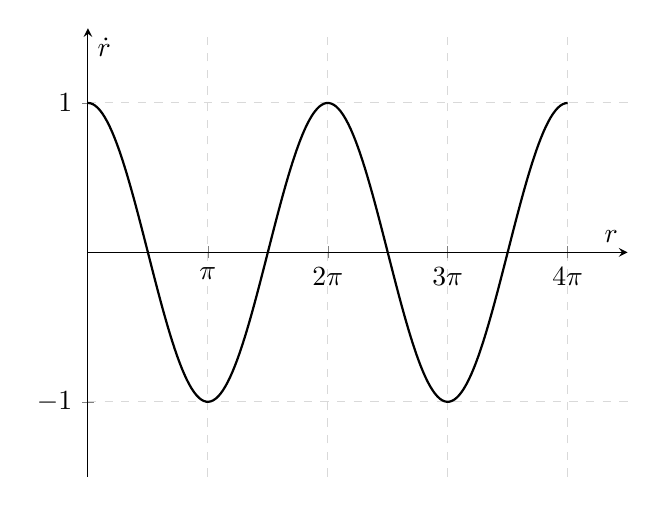
\begin{tikzpicture}
    \begin{axis}[
        domain=0:4*pi,
        samples=200,
        axis lines=middle,
        xlabel={$r$},
        ylabel={$\dot{r}$},
        xtick={0, pi, 2*pi, 3*pi, 4*pi},
        xticklabels={$0$, $\pi$, $2\pi$, $3\pi$, $4\pi$},
        ytick={-1, 0, 1},
        ymin=-1.5, ymax=1.5,
        xmin=0, xmax=4.5*pi,
        grid=both,
        grid style={dashed, gray!30},
    ]
        \addplot[black, thick] {cos(deg(x))};
    \end{axis}
\end{tikzpicture}



Now we look at the sign of $\dot{r}$ near each limit cycle:

So, $\frac{3\pi}{2}:$ 

\begin{align*}
    r&<\frac{3\pi}{2} \implies \dot{r} 
< 0 \ \text{spirals in towards circle $r = \frac{\pi}{2}$} \\
r&>\frac{3\pi}{2} \implies \dot{r}
> 0  \ \text{spirals out towards circle $r = \frac{5\pi}{2}$}\\
\dot{\theta}&>0 \ \text{so motion is anticlockwise}
\end{align*}



Now, $\frac{5\pi}{2}:$ 

\begin{align*}
    r&<\frac{5\pi}{2} \implies \dot{r}
> 0 \ \text{spirals out towards circle $r = \frac{5\pi}{2}$}\\
r&>\frac{5\pi}{2} \implies \dot{r}
< 0 \ \text{spirals in towards circle $r = \frac{5\pi}{2}$} \\
\dot{\theta}&>0 \ \text{so motion is anticlockwise}
\end{align*}\\

Due to periodicity of $\cos$ we know that for $r = \displaystyle\frac{(2n+1)\pi}{2}$, if we have even $n$ it is stable, and for odd $n$ it is unstable

\subsubsection{Laplace Questions}

Find the inverse Laplace transform of
\begin{itemize}
    \item[i.] \( F(s) = \frac{e^{-2s}}{s^2 + s - 2} \),
    \item[ii.] \( F(s) = \frac{(s - 2) e^{-s}}{s^2 - 4s + 3} \).
\end{itemize}

\textbf{Solution:} We use the identity\\
\[
\mathcal{L}^{-1}\{ e^{-cs} F(s) \} = u_c(t) f(t - c) \quad \text{with } f(t) = \mathcal{L}^{-1}\{ F(s) \}.
\]

\textbf{i.} Consider \( F(s) = \frac{e^{-2s}}{s^2 + s - 2} \). Using the identity above and the decomposition\\
\[
\frac{1}{s^2 + s - 2} = \frac{1}{3} \frac{1}{s - 1} - \frac{1}{3} \frac{1}{s + 2},
\]
we find\\
\[
\mathcal{L}^{-1}\left\{ \frac{1}{s^2 + s - 2} \right\} = \frac{1}{3} \left( e^t - e^{-2t} \right).
\]
Thus, the overall inverse Laplace transform equals\\
\[
\mathcal{L}^{-1}\left\{ \frac{e^{-2s}}{s^2 + s - 2} \right\} = u_2(t) \frac{1}{3} \left( e^{t-2} - e^{-2(t-2)} \right).
\]

\textbf{ii.} Consider \( F(s) = \frac{(s - 2) e^{-s}}{s^2 - 4s + 3} \). Similarly, we now compute the Laplace inverse of\\
\[
\frac{s - 2}{s^2 - 4s + 3} = \frac{s - 2}{(s - 2)^2 - 1},
\]
to obtain\\
\[
\mathcal{L}^{-1}\left\{ \frac{s - 2}{s^2 - 4s + 3} \right\} = e^{2t} \cosh t.
\]
Thus, the overall inverse Laplace transform equals\\
\[
\mathcal{L}^{-1}\left\{ \frac{(s - 2) e^{-s}}{s^2 - 4s + 3} \right\} = u_1(t) e^{2(t-1)} \cosh(t - 1).
\]

\bigskip
\textbf{Find the general solution to the following initial-value problem using Laplace transforms:}

\begin{itemize}
    \item[i.] \( y'' + 2y' + 2y = h(t), \quad y(0) = 0, \quad y'(0) = 1, \)
    where\\
    \[
    h(t) =
    \begin{cases}
        1, & \pi \le t < 2\pi, \\
        0, & 0 \le t < \pi \text{ or } t \ge 2\pi.
    \end{cases}
    \]
\end{itemize}

Compute the Laplace transform of \( y'' + 2y' + 2y = h(t) \) using the fact that \( h(t) = u_\pi(t) - u_{2\pi}(t) \). \\

We obtain\\
\[
s^2 Y(s) - s y(0) - y'(0) + 2 \left( s Y(s) - y(0) \right) + 2 Y(s) = \frac{e^{-\pi s}}{s} - \frac{e^{-2\pi s}}{s}.
\]
Using the initial conditions \( y(0) = 0 \), \( y'(0) = 1 \), we solve for \( Y(s) \),\\
\[
Y(s) = \frac{e^{-\pi s}}{s(s^2 + 2s + 2)} - \frac{e^{-2\pi s}}{s(s^2 + 2s + 2)} + \frac{1}{s^2 + 2s + 2}.
\]
The last step is to compute the Laplace inverse of \( Y(s) \). Using linearity and\\
\[
y(t) = f(t) + u_\pi(t) g(t - \pi) - u_{2\pi}(t) g(t - 2\pi),
\]
where\\
\[
f(t) = \mathcal{L}^{-1}\left\{ \frac{1}{s^2 + 2s + 2} \right\}, \quad g(t) = \mathcal{L}^{-1}\left\{ \frac{1}{s(s^2 + 2s + 2)} \right\}.
\]
Consider the first fraction,\\
\[
\frac{1}{s^2 + 2s + 2} = \frac{1}{(s + 1)^2 + 1} \quad \Rightarrow \quad f(t) = e^{-t} \sin t.
\]
Consider the second fraction,\\
\[
\frac{1}{s(s^2 + 2s + 2)} = \frac{1}{2s} - \frac{s}{2} + \frac{1}{(s + 1)^2 + 1} \]\\\[= \frac{1}{2} \left( \frac{1}{s} - \frac{s}{(s + 1)^2 + 1} - \frac{1}{(s + 1)^2 + 1} \right).
\]
We can compute its Laplace inverse, giving rise to\\
\[
g(t) = \frac{1}{2} \left( 1 - e^{-t} \cos t - e^{-t} \sin t \right).
\]
We conclude that\\
\[
y(t) = e^{-t} \sin t + \frac{1}{2} u_\pi(t) \left( 1 + e^{-(t-\pi)} \cos t + e^{-(t-\pi)} \sin t \right)\]\\\[ - \frac{1}{2} u_{2\pi}(t) \left( 1 - e^{-(t-2\pi)} \cos t - e^{-(t-2\pi)} \sin t \right),
\]
where we used that \( \cos(t - \pi) = - \cos t \), \( \sin(t - \pi) = - \sin t \), \( \cos(t - 2\pi) = \cos t \), and \( \sin(t - 2\pi) = \sin t \).


\bigskip
\newpage
\textbf{Consider the Volterra equation}\\
\[
y(t) + \int_0^t (t - x) y(x) \, dx = - \frac{1}{4} \sin(2t).
\]
i. Solve this integral equation using the Laplace transform.

\textbf{Solution:}

Taking the Laplace transform of the integral equation, using the convolution
theorem and that \( L\{t\}(s) = \frac{1}{s^2} \), we find\\
\[
Y(s) + \frac{Y(s)}{s^2} = - \frac{1}{2(s^2 + 4)}.
\]
This uses that \( y(0) = 0 \) as follows from the integral equation. Solving for \( Y(s) \), we have
\\\[
Y(s) = - \frac{s^2}{2(s^2 + 1)(s^2 + 4)},
\]
and after some manipulations,\\
\[
Y(s) = \frac{1}{6} \cdot \frac{1}{s^2 + 1} - \frac{2}{3} \cdot \frac{1}{s^2 + 4}.
\]
Thus, the solution is\\
\[
y(t) = \frac{1}{6} \sin t - \frac{1}{3} \sin(2t).
\]

\subsubsection{Convolution}
Find the inverse Laplace transform of the functions
\begin{enumerate}
    \item[i.] \( H_1(s) = \frac{s}{(s + 1)(s^2 + 4)} \) and
    \item[ii.] \( H_2(s) = \frac{G(s)}{s^2 + 1} \)
\end{enumerate}
using the convolution theorem.

\textbf{Solution:}

i. We write \( H_1(s) = F(s)G(s) \) with \( F(s) = \frac{1}{s + 1} \) and \( G(s) = \frac{s}{s^2 + 4} \) so that \( f(t) = e^{-t} \) and \( g(t) = \cos(2t) \), leading to the inverse transform\\
\[
h_1(t) = \int_0^t e^{-(t-\tau)} \cos(2\tau) \, d\tau.
\]

ii. We write \( H_2(s) = F(s)G(s) \) with \( F(s) = \frac{1}{s^2 + 1} \) so that \( f(t) = \sin t \), leading to\\
\[
h_2(t) = \int_0^t \sin(t - \tau) g(\tau) \, d\tau.
\]


\end{multicols}

\Large
\subsection{LAPLACE TABLE}
\bigskip
    \[
\begin{array}{|c|c|c|c|c|}
\hline
f(t) & F(t) := \mathcal{L}\{f\}(s) & f(t) & F(t) := \mathcal{L}\{f\}(s) \\
\hline
1 & \frac{1}{s} & e^{at} \sin(bt) & \frac{b}{(s-a)^2+b^2}\\
e^{at} & \frac{1}{s-a} & e^{at} \cos(bt) & \frac{s-a}{(s-a)^2+b^2}\\
t^n & \frac{n!}{s^{n+1}} & e^{at} t^n & \frac{n!}{(s-a)^{n+1}}\\
\sin(at) & \frac{a}{s^2 + a^2} & u_c(t) & \frac{e^{-cs}}{s}\\
\cos(at) & \frac{s}{s^2 + a^2} & \delta(t-c) & \lim_{\alpha\to c}(e^{-\alpha s})\\
\sinh(at) & \frac{a}{s^2 - a^2} & f^{(n)}(t) & s^nF(s)-\sum_{k=1}^{n-1} s^{n-k} f^{(k)}(0)\\
\cosh(at) & \frac{s}{s^2 - a^2} & (-t)^n f(t)& F^{(n)}(s) \\
f(t)& \int_0^\infty e^{-st}f(t)dt & u_c(t) f(t-c) & e^{-cs}F(s)\\
\hline
\end{array}
\]
\subsection{CRITICAL POINTS}
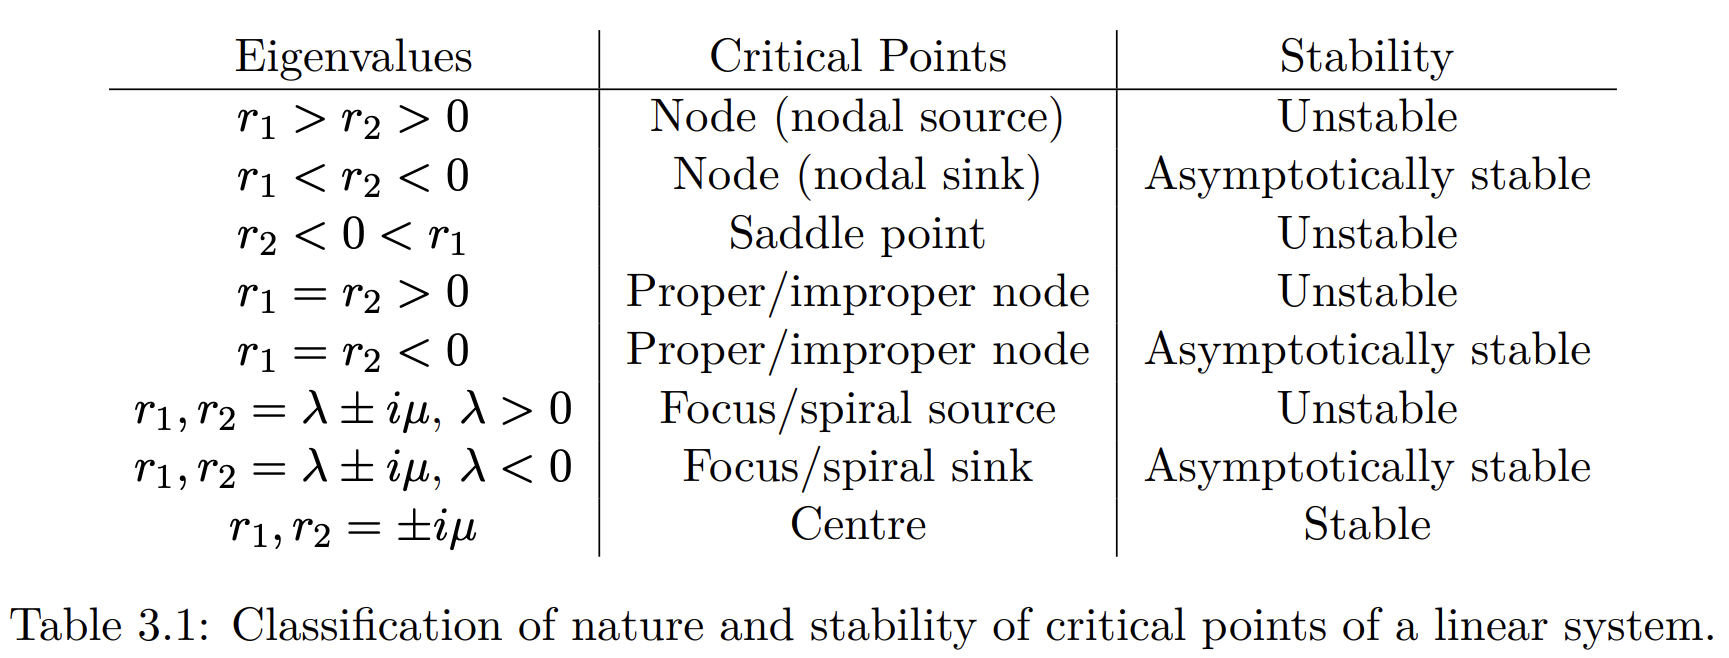
\includegraphics[width = 18 cm]{CritPtsTable.png}





\end{document}
